%!TEX root=./LIVRO.tex

\chapter{O gênero fábula}
\markboth{Módulo 1}{}

%  \coment{Neste módulo, por meio do trabalho com o gênero textual fábula,
%   espera-se que os alunos consigam localizar informações explícitas, inferir
%   informações implícitas, inferir o sentido de palavras ou expressões e
%   reconhecer o significado de palavras derivadas com base em seus afixos.}

\section*{Habilidades do SAEB}

\begin{itemize}
  \item Identificar a ideia central do texto.
  \item Localizar informação explícita.
  \item Inferir informações implícitas em textos.
  \item Inferir o sentido de palavras ou expressões em textos.
  \item Reconhecer em textos o significado de palavras derivadas a partir de
seus afixos.
\end{itemize}

\subsection*{Habilidades da BNCC}

\begin{itemize}
  \item EF35LP03, EF15LP03, EF35LP04, EF35LP05, EF03LP10.
\end{itemize}

\conteudo{{\hfill\textbf{Fábulas}\hfill}\medskip

Histórias que têm animais como personagens existem há muito tempo. Você
já leu ou escutou alguma história na qual os animais se comportam como
seres humanos?

As fábulas são narrativas com essas características, com personagens
como animais, plantas ou objetos, aos quais são atribuídas características humanas. Elas 
geralmente apresentam, no final, um ensinamento, uma moral ou um conselho, chamado
de \textit{moral da história}.

Esopo, que viveu na Grécia Antiga, é autor de diversos textos desse
gênero.

\begin{center}
\noindent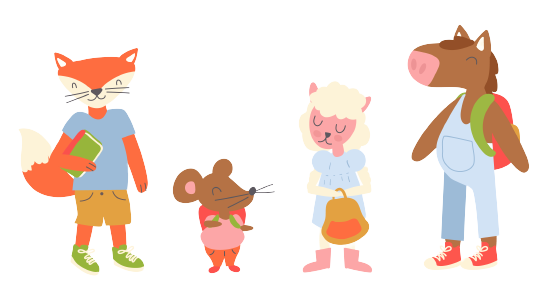
\includegraphics[width=.9\textwidth]{./media/image1a.png}
\end{center}

As fábulas são consideradas um gênero literário e são uma das mais
antigas formas de se contar uma história. Elas podem ser escritas
em prosa (texto em parágrafos) ou em versos. Os títulos normalmente se
referem às personagens, e o tempo e o espaço relacionam-se ao ambiente
delas. A linguagem é simples, objetiva e direta.        
}

\section*{Atividades}

Leia, agora, a adaptação de uma fábula de Esopo.

%\coment{Oriente os alunos a realizar, primeiramente, a leitura silenciosa do
  % texto, seguida de leitura em voz alta. Essa estratégia de leitura
  % possibilita que o aluno desenvolva fluência leitora, facilitando a
  % compreensão global do texto lido. As atividades introdutórias são de
  % compreensão do texto e têm a finalidade de desenvolver habilidades de
  % constatar, localizar informações, realizar simples inferências, deduzir
  % significados de termos do texto e inferir o tempo em que ocorre a
  % narrativa.}

\begin{myquote}
\textbf{O leão e a pulga}\medskip

O leão acordou incomodado por algo. Depois de alguns instantes, notou que uma pulga o mordia. A pulga sorria satisfeita. 

--- Não tenho medo do leão por causa da sua larga juba -- disse a pulga, enquanto mordia o focinho do leão.  

\begin{center}
\noindent
\includegraphics[width=.9\textwidth]{./media/image1b.png}
\end{center}

Irritado com a mordida da pulga, o leão deu um duro golpe contra o próprio focinho, e outro, e outro, e outro. Mas isso criou uma ferida no leão que urrou como um louco.

Quando a pulga foi embora, queria contar a todos como tinha vencido o leão. Porém, antes de contar a qualquer um, caiu na teia de uma aranha minúscula que a devorou. \\

\noindent\textsc{\textbf{moral da história}}: Muitas vezes o menor de nossos inimigos é o mais terrível.

\fonte{Texto adaptado para este material.}
\end{myquote}

\num{1} Quem são as personagens da fábula?

\reduline{O leão, a pulga e a aranha.\hfill}
\linhas{1}

\num{2} Por que o leão ficou irritado?

\reduline{O leão ficou irritado porque a pulga picou seu focinho.\hfill}
\linhas{1}

\num{3} O que houve com a pulga finalmente?

\reduline{A pulga foi comida por uma aranha minúscula.\hfill}
\linhas{3}

\num{4} Em sua opinião, onde ocorreu a história?

\reduline{É provável que os alunos respondam que a história pode ter ocorrido na floresta.\hfill}
\linhas{3}

\num{5} Qual é a moral da história? Transcreva no espaço a seguir.

\reduline{Muitas vezes o menor de nossos inimigos é o mais terrível.\hfill}
\linhas{3}

\num{6} Reescreva as frases a seguir, trocando as palavras em destaque por
sinônimos, ou seja, palavras diferentes que têm significado
semelhante.

%\coment{Para o desenvolvimento desta atividade, coloque à disposição dos alunos diferentes dicionários para consulta.}

\begin{escolha}[itemsep=-5pt]
\item Mas isso criou uma ferida no leão que \textbf{\underline{urrou}} como um louco.
\reduline{Sugestão de resposta: Mas isso criou uma ferida no leão que \textbf{rugiu} como um louco.\hfill}

\linhas{3}

\item \textbf{\underline{Irritado}} com a mordida da pulga, o leão deu um duro golpe contra o próprio focinho, e outro, e outro, e outro.
\reduline{Sugestão de resposta: \textbf{Bravo} com a mordida da pulga, o leão deu um duro golpe contra o próprio focinho, e outro, e outro, e outro.\hfill}
\linhas{2}

\item Porém, antes de contar a qualquer um, caiu na teia de uma aranha \textbf{\underline{minúscula}} que a devorou.
\reduline{Sugestão de resposta: Porém, antes de contar a qualquer um, caiu na teia de uma aranha \textbf{pequenina} que a devorou.\hfill}
\linhas{2}
\end{escolha}

\num{7} Caracterize com suas palavras a atitude da pulga.

\reduline{Era arrogante e queria provar que era mais corajosa que o leão.\hfill}
\linhas{2}

\num{8} Muitas palavras são formadas a partir de outras. As que são formadas são
palavras \textbf{derivadas} de outras palavras, que são denominadas
\textbf{primitivas}. Observe o quadro a seguir e, em seguida, faça as
atividades propostas.

\begin{center}
\begin{tabular}{c|c}
\hline
\textbf{Palavra primitiva} & \textbf{Palavra derivada} \\ \hline
\rowcolor{blue!20} Livro & Livraria\\
Flor & Floreira\\
\rowcolor{blue!30} Medo & Medroso\\ \hline
\end{tabular}
\end{center}

Separe as palavras a seguir em sílabas e escreva um substantivo ou um
adjetivo derivado para cada uma delas.

\begin{escolha}[itemsep=-5pt]
\item Leite: \reduline{lei-te\hfill}
\reduline{leiteiro\hfill}
\item
  Barba: \reduline{bar-ba\hfill}
\reduline{barbeiro\hfill}
\item
  Saco: \reduline{sa-co\hfill}
\reduline{sacola\hfill}
\item
  Pedra: \reduline{pe-dra\hfill}
\reduline{pedreiro\hfill}

 % Manteiga: \reduline{man-tei-ga\hfill}
%\reduline{amanteigado\hfill}
\end{escolha}

\num{9} Escreva o substantivo primitivo das palavras a seguir.

\begin{escolha}[itemsep=-5pt]
\item Boleira: \reduline{bolo\hfill}

\item Beleza: \reduline{belo\hfill}

\item Cabeluda: \reduline{cabelo\hfill}

\item Mangueira: \reduline{manga\hfill}

\end{escolha}

\num{10} Ligue cada palavra derivada à respectiva palavra primitiva.

\begin{center}
\begin{multicols}{2}
\red{Empedrado} 

\red{Padeiro} 

\red{Macieira} 

\red{Apimentada}

\blue{Maçã}

\blue{Pimenta}

\blue{Pedra}

\blue{Pão}
\end{multicols}
\end{center}

\coment{Empedrado está ligado à pedra; padeiro, a pão; macieira, à maçã; apimentado, à pimenta.}

\num{11} Você lembra o que são sinônimos e antônimos? Leia o quadro para
relembrar.

%\coment{Estas atividades facilitam o desenvolvimento da habilidade de inferir significados de palavras desconhecidas sem recorrer ao dicionário.}

\begin{longtable}[]{@{}l@{}}
\toprule
\begin{minipage}[t]{0.97\columnwidth}\raggedright\strut
\textbf{Sinônimo}: palavra que apresenta significado semelhante ao de
outra.

\textbf{Antônimo}: palavra que apresenta significado contrário ao de
outra.
\strut
\end{minipage}\tabularnewline
\bottomrule
\end{longtable}

\begin{escolha}[itemsep=-5pt]
\item Leia a frase a seguir e marque as palavras que poderiam substituir aquelas que estão em destaque por terem significados semelhantes.

O leão estava \textbf{triste} e \textbf{fraco}.

\begin{minipage}{.4\textwidth}
\begin{boxlist}
\boxitem{X} infeliz -- debilitado
\boxitem{\white{X}} feliz -- sadio
\boxitem{\white{X}} ágil -- robusto
\boxitem{\white{X}} saltitante -- forte
\end{boxlist}
\end{minipage}\vspace*{.5cm}
\begin{minipage}{.5\textwidth}

\includegraphics[width=.6\textwidth]{./media/image1c.png}
\end{minipage}

\item Escreva palavras antônimas de

\begin{itemize}
\item
  moderno: \reduline{antigo\hfill}
\item
  quente: \reduline{frio\hfill}
\item
  dia: \reduline{noite\hfill}
\item
  dentro: \reduline{fora\hfill}
\item
  claro: \reduline{escuro\hfill}
\item
  cair: \reduline{levantar\hfill}
\end{itemize}
\end{escolha}

\pagebreak
\num{12} No caça-palavra a seguir, encontre palavras com sentido contrário aos das palavras do quadro.

\begin{myquote}
\textbf{sair}\hfill \textbf{abrir}\hfill \textbf{descer}\hfill \textbf{acordar}\hfill \textbf{branco}\hfill \textbf{bonito}\hfill
\end{myquote}

\begin{center}
\begin{tabular}{llllllllllll}
E & T & E & E & W & D & T & T & B & H & L & U\\

A & F & N & I & A & N & E & H & I & S & D & D\\

O & E & E & I & D & I & O & P & E & R & E & C\\

H & I & D & C & S & T & E & N & H & E & A & E\\

H & O & N & U & H & D & N & O & S & E & A & J\\

D & V & B & M & Y & A & T & P & E & Y & M & N\\

Y & I & U & F & C & R & R & W & D & R & O & F\\

R & H & D & C & T & E & A & O & O & E & O & I\\

O & T & D & A & T & S & R & O & H & N & T & A\\

Y & C & E & O & L & F & D & O & R & M & I & R\\

D & V & M & U & O & T & S & E & C & S & S & N\\

E & T & H & H & A & Y & L & R & E & L & F & S
\end{tabular}
\end{center}
%NOTE. Colocar as respostas em magenta.

\num{13} É possível formar antônimos usando \textbf{prefixos}, ou seja, pequenas
partes de palavras usadas antes das palavras primitivas. Observe os exemplos a seguir.

\begin{myquote}
\centering
Feliz -- \textbf{In}feliz

Fazer -- \textbf{Des}fazer
\end{myquote}

Acrescente \textbf{in-}, \textbf{im-} ou \textbf{des-} às palavras a seguir e crie antônimos.

\begin{escolha}[itemsep=-5pt]
\item Ligar: \reduline{desligar\hfill}

\item Próprio: \reduline{impróprio\hfill}

%\item Afogar: \reduline{desafogar\hfill}

\item Satisfeito: \reduline{insatisfeito\hfill}

%\item Amar: \reduline{desamar\hfill}

%\item Iludir: \reduline{desiludir\hfill}

%\item Parcial: \reduline{imparcial\hfill}

%\item Preparada: \reduline{despreparada\hfill}
\end{escolha}


\pagebreak
\section*{Treino}

\num{1} Leia a fábula.

\begin{myquote}
\textbf{O ratinho, o gato e o galo}

Certa manhã, um ratinho saiu do buraco pela primeira vez. Queria
conhecer o mundo e travar relações com tanta coisa bonita de que falavam
seus amigos. Admirou a luz do sol, o verdor das árvores, a correnteza
dos rios, a habitação dos homens. E acabou entrando no quintal duma casa
da roça.

\begin{center}
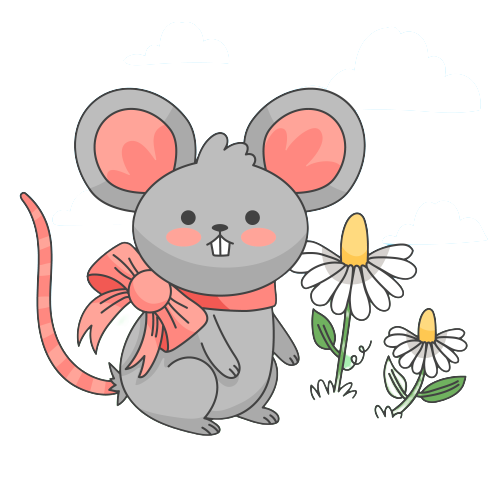
\includegraphics[width=.5\textwidth]{./media/image1d.png}
\end{center}

--- Sim, senhor! É interessante isto!

Examinou tudo minuciosamente, farejou a tulha de milho e a estrebaria.
Em seguida, notou no terreiro um certo animal de belo pelo, que dormia
sossegado ao sol. Aproximou-se dele e farejou-o, sem
receio nenhum. Nisto, aparece um galo, que bate as asas e canta.
{[}...{]}.

\fonte{O ratinho, o gato e o galo. Disponível em:
\emph{http://www.dominiopublico.gov.br/download/texto/me000589.pdf}. Acesso em:
14 fev. 2023.}
\end{myquote}
%NOTE. Ir até a USP procurar o volume Fábulas de Monteiro Lobato e bater o texto, se ele existir.

\pagebreak
Onde a segunda parte da história se passa?

\begin{escolha}[itemsep=-5pt]
\item No buraco dos ratinhos.

\item Em uma árvore do campo.

\item Em um rio com correnteza.

\item Em um espaço de roça.
\end{escolha}


\num{2} Leia a fábula e responda ao que se pede a seguir.

\begin{myquote}
\textbf{A raposa e as uvas} \bigskip 

Certa raposa esfaimada encontrou uma parreira carregadinha de lindos cachos maduros, coisa de fazer vir água à boca. Mas alta, tão alta que nem pulando podia colher um bago só.

O matreiro bicho, torcendo o focinho, disse com desprezo:

\begin{center}
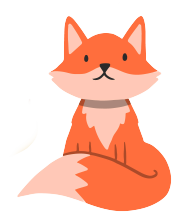
\includegraphics[width=.2\textwidth]{./media/image1e.png}
\end{center}

--- Estão verdes. Uvas assim só os cães podem tragar.

E foi-se. Nisto deu um vento e uma folha tombou. A raposa ouvindo o barulho, e julgando ser um bago, volta a toda a pressa e põe-se a farejar... \medskip

\noindent\textsc{\textbf{moral da história}}: Quem desdenha quer comprar.

\fonte{Monteiro Lobato. \textit{Fábulas de Narizinho}. São Paulo: Monteiro Lobato \& Cia, 1921. p. 39. Adaptado.}
\end{myquote}
%Note. Conferir gabarito de acordo com o novo exercício.

\noindent Que palavra a seguir apresenta sentido semelhante ao da palavra
``matreiro'', do texto?

\begin{escolha}[itemsep=-5pt]
\item Destemido.

\item Covarde.

\item Esperto.

\item Doido.
\end{escolha}

\num{3} Leia a fábula e responda.

\begin{myquote}
\begin{minipage}{.9\textwidth}
\begin{verse}
\textbf{A cigarra e a formiga}

No verão, a cigarra cantou,\\
Mas quando mudou o vento,\\
E ela se viu sem alimento,\\ 
Na casa ao lado, chorou,\\
Pedindo à formiga, humildemente:\\

--- Dá-me um grão até a primavera.\\
Lhe devolvo, disse ela.\\
Surpresa, a formiga disse:\\

--- O que fazia no tempo quente?\\
Cantava noite e dia? Fico contente.\\Cantou, agora dance, suspirou.\\

\fonte{Adaptação livre da fábula ``A cigarra e a formiga'' de La Fontaine.}
\end{verse}
\end{minipage}
\begin{minipage}{.1\textwidth}
\end{minipage}
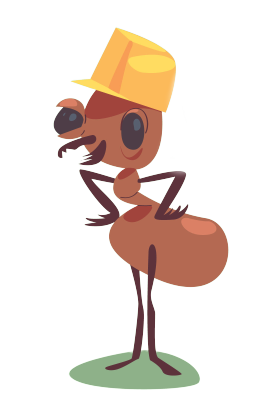
\includegraphics[width=.2\textwidth]{./media/image1f.png}
\end{myquote}

A palavra ``humildemente'' é classificada como

\begin{escolha}[itemsep=-5pt]
\item primitiva, pois é possível formar outras palavras a partir dela.

\item derivada, pois foi formada a partir de uma palavra primitiva.

\item derivada, pois não apresenta relação com outras palavras.

\item primitiva, pois é uma palavra que não deriva de outras.
\end{escolha}
%Note. Conferir gabarito de acordo com o novo exercício.

\chapter{O texto teatral}
\markboth{Módulo 2}{}

%\coment{Neste módulo, será abordado o texto dramático, seu contexto de produção e circulação, além de sua forma composicional. Espera-se que os alunos leiam e compreendam texto do campo artístico-literário; reconheçam o tema principal do texto; percebam o enredo expresso em textos dramáticos; localizem informações explícitas no texto dramático; infiram o sentido de palavras no texto, com base no contexto de trecho do texto; assim como analisem os efeitos de sentido de verbos de enunciação.}

\section*{Habilidades do SAEB}

\begin{itemize}
  \item Reconhecer diferentes gêneros textuais.
  \item Identificar elementos constitutivos de textos narrativos.
  \item Identificar as marcas de organização de textos dramáticos.
  \item Analisar os efeitos de sentido de verbos de enunciação.
\end{itemize}

\subsection{Habilidades da BNCC}

\begin{itemize}
  \item EF35LP03, EF15LP03, EF35LP04, EF35LP05, EF03LP10.
\end{itemize}

\conteudo{
%https://www.pexels.com/pt-br/foto/agindo-atuacao-substituto-irmao-5801566/

\begin{wrapfigure}{l}{.4\textwidth}
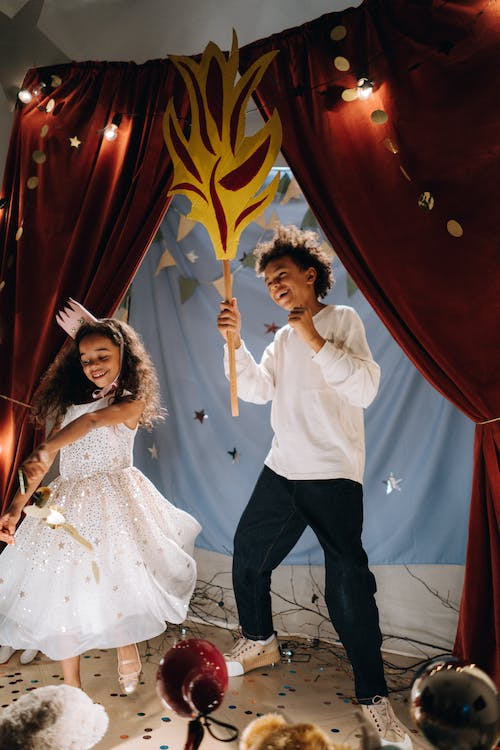
\includegraphics[width=1.8in,height=2.8in]{./media/image1.jpeg}
\end{wrapfigure}

Uma história para ser encenada no teatro tem características próprias.
Como em um \textbf{roteiro}, o texto teatral apresenta uma estrutura adequada para
ser utilizada pelo diretor, pelos atores e pela equipe técnica na hora da encenação.

Geralmente, ele apresenta os seguintes elementos: 
título, lista de personagens, organização em atos e cenas, 
diálogos, que constitui a maior parte do texto, e pode ter rubricas.

As rubricas são instruções de como uma cena deve ser composta. 
Podem indicar movimentos, expressões faciais, gestos, 
figurino, cenário, iluminação, música, entre outros elementos.

No teatro, a história é transmitida por meio de ações e
diálogos das personagens, que são representados por
atores. 
}


\section*{Atividades}

Leia o trecho da peça teatral para resolver os itens de 1 a 6.

%\coment{Realize uma leitura compartilhada do texto. Chame a atenção dos alunos para as rubricas no texto e para sua função de orientar a dramatização (como indicações das formas de falar, caminhar, gesticular; indicação de características como altura da voz, ritmo). Solicite aos alunos que observem quem são os personagens e qual é o papel de cada um.}

%Inserir imagem ao lado do texto:
%https://pixabay.com/pt/vectors/violino-violinista-banda-bandsman-154220/

\begin{myquote}
\textbf{Zé Betovi e Nhô Mozarte}

\textit{(Entra Nhô Mozarte com seu livro embaixo do braço olhando em
sua volta e fala em voz alta:)}
\vspace{1ex}

\textsc{Nhô Mozarte}: Aqui está bem mais tranquilo. Pelo menos não tem
nenhuma obra por perto. Com aquele barulho danado das máquinas, eu não
estava conseguindo me concentrar.

\vspace{1ex}
\textit{(Em seguida, senta-se no banco da praça e começa a ler.)}
\vspace{1ex}

%NOTE. LaTeX. Melhorar diagramação, com problema no myquote.

\textsc{Zé Betovi}: Tchau, mãe! Tô indo lá na praça tocar um pouco.

\begin{wrapfigure}{r}{.4\textwidth}
\centering
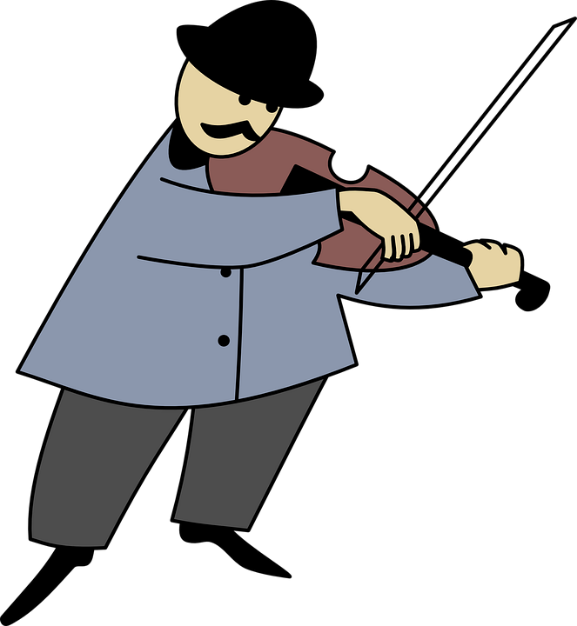
\includegraphics[width=1.7in,height=1.7in]{./media/image2.png}
\end{wrapfigure}

\vspace{1ex}
\textit{(Zé Betovi caminha em
direção à praça com seu violino na mão e resolve se sentar perto de uma
árvore, pois o calor estava muito grande naquele dia. Nem notou a
presença de Nhô Mozarte sentado no banco, entretido lendo seu livro, e
começa a tocar. Quando Nhô Mozarte escuta a música, para de ler e
procura ver de onde vem aquele som. Avista Zé Betovi sentado tocando.
Então se levanta devagar, procurando não fazer barulho, e vai em direção
a ele. Quando Zé Betovi acaba de tocar, aplaude com entusiasmo.)}
\vspace{1ex}

\textsc{Nhô Mozarte}: Bravo, meu jovem! Que maravilha! Estou admirado de
ver um garoto de sua idade tocando violino. E um instrumento que não é
fácil. Os jovens assim como você, principalmente nos dias de hoje,
preferem as guitarras, baterias, violão.

\textsc{Zé Betovi}: Obrigado. É mesmo... Eu também gosto dos outros
instrumentos. Tenho violão e teclado e toco de vez em quando, mas o meu
preferido mesmo é esse aqui. \textit{(Mostra o violino.)}

\textsc{Nhô Mozarte}: Um artista completo! \textit{(Expressa admiração.)} Então, se
você toca violino, é porque aprecia a música clássica.

\textsc{Zé Betovi}: Gosto. E nem tinha como eu não gostar. Lá em casa
tanto meu pai como minha mãe adoram. Na verdade, eu cresci ouvindo. Meu
avô, o pai de minha mãe, tocava muito bem de ouvido e nem sabia ler
partitura.

\textsc{Nhô Mozarte}: E você? Toca de ouvido como seu avô?

\textsc{Zé Betovi}: Das duas formas. Minha mãe me colocou em aulas de
música desde que eu era bem pequeno. Ela achou que ia ser bom pra mim.
E, quando eu fiz seis anos, escolhi o violino.

\textsc{Nhô Mozarte}: Sua mãe fez muito bem. A música é importante na vida
de todo mundo. Ela nos ajuda em tantas coisas... Mas me diga, meu rapaz:
você sabe quem é o autor da música que estava tocando há pouco?

\textsc{Zé Betovi}: Villa-Lobos.

{[}...{]}

\fonte{Marluzi Moreira de Carvalho. Teatro na escola. Zé Betovi e Nhô Mozarte.
Disponível em:
\emph{www.teatronaescola.com/index.php/banco-de-pecas/category/infantil-ou-infanto-juvenil-2}.
Acesso em: 15 fev. 2023. (Adaptado.)}
\end{myquote}

\pagebreak
\num{1} Quem são os personagens desse texto? 

\reduline{Zé Betovi e Nhô Mozarte.\hfill}
\linhas{1}

\num{2} As rubricas no texto servem para orientar a dramatização. Sublinhe cada uma delas.
\bigskip

\num{3} Qual é o instrumento preferido de Zé Betovi? 

\reduline{O violino.\hfill}
\linhas{1}

\num{4} Os nomes dos personagens foram inspirados em dois músicos famosos. Você
consegue identificar quem são eles? 

\reduline{Mozart e Beethoven.\hfill}
\linhas{1}

\num{5} O texto apresentado é teatral. Com qual objetivo esses textos são
escritos? 

\reduline{O objetivo de se escrever textos desse tipo é que sejam encenados.\hfill}
\linhas{1}


\num{6} Releia o trecho a seguir.

\begin{myquote}
\textsc{Nhô Mozarte}: Bravo, meu jovem! Que maravilha! Estou admirado de
ver um garoto de sua idade tocando violino. {[}...{]} Os jovens assim
como você, principalmente nos dias de hoje, preferem as
\textbf{guitarras}, \textbf{baterias}, \textbf{violão}.
\end{myquote}

No espaço a seguir, faça um desenho de cada instrumento musical
destacado e escreva o nome de cada um deles abaixo do respectivo desenho.

\begin{mdframed}[linewidth=2pt,linecolor=salmao,roundcorner=20pt]
\vspace{12cm}
\end{mdframed}

No conto ``João e Maria'', narra-se a história de dois irmãos que são
abandonados pelo pai e pela madrasta na floresta. Leia um trecho desse
conto e resolva as atividade de 7 a 13.

%Inserir imagem de floresta: https://unsplash.com/pt-br/fotografias/6YHlHIVROzg

\begin{myquote}
\textbf{João e Maria}

Às margens de uma extensa mata, existia, há muito tempo, uma cabana
pobre, feita de troncos de árvore, na qual morava um lenhador com sua segunda esposa e
seus dois filhinhos, nascidos do primeiro casamento. O garoto chamava-se João, e a
menina, Maria.

A vida sempre fora difícil na casa do lenhador, mas naquela época as
coisas haviam piorado ainda mais: não havia pão para todos.

\vspace{2ex}
\begin{center}
\noindent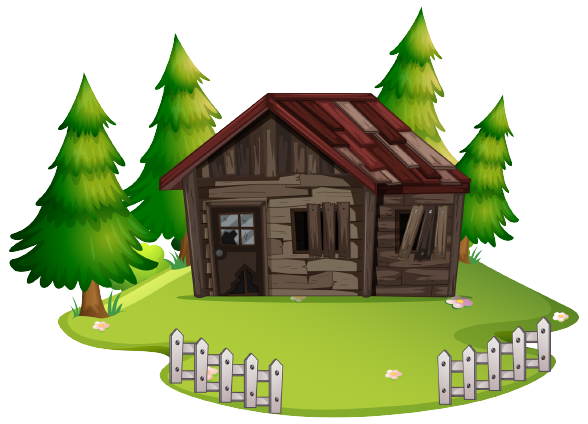
\includegraphics[width=\textwidth]{./media/image3a.png}
\end{center}

--- Minha mulher, o que será de nós? Acabaremos todos por morrer
de necessidade. E as crianças serão as primeiras.

--- Há uma solução --- disse a madrasta, que era muito
malvada. --- Amanhã, daremos a João e Maria um pedaço de pão, depois os
levaremos à mata e lá os abandonaremos.

{[}...{]}

\fonte{Irmãos Grimm. João e Maria. Disponível em:
\emph{www.dominiopublico.gov.br/download/texto/me000589.pdf}. Acesso em: 15
fev. 2023.}
\end{myquote}

\num{7} Faça o que se pede a seguir.

\begin{escolha}[itemsep=-5pt]
\item Indique quem são as personagens dessa história.
\reduline{João, Maria, o pai e a madrasta.\hfill}

\item Explique por que a madrasta sugeriu abandonar João e Maria.
\reduline{A madrasta deu essa sugestão, porque não havia comida para todos.\hfill}

\pagebreak
\item Indique onde os pais planejavam abandonar as crianças.
\reduline{Eles planejavam abandonar as crianças na mata.\hfill}
\end{escolha}

% \item Marque a alternativa correta em relação ao que mostra o trecho
% selecionado do conto ``João e Maria''.

% \begin{boxlist}
% \boxitem{\white{X}} A situação de tristeza que tomou conta do pai e da madrasta depois
% de eles abandonarem as crianças.

% \boxitem{X} Os motivos que levaram o pai e a madrasta a pensarem em deixar as
% crianças na floresta.
% \end{boxlist}
% \end{escolha}

\num{8} Releia a história e sublinhe no texto:

\begin{escolha}[itemsep=-5pt]
\item de vermelho, a fala do pai.

\item de verde, a fala da madrasta.
\end{escolha}

\num{9} Narrador é aquele que conta a história. Transcreva uma frase do texto que
pertence ao narrador.

\reduline{Os alunos podem dar respostas diferentes para este item. ``O garoto chamava-se João, e a menina, Maria.'' é uma das possibilidades.\hfill}
\linhas{1}

%NOTE. LaTeX. Problema nas aspas tipográficas. ``João e Maria''


% \begin{escolha}[itemsep=-5pt]
% \boxitem{X} O garoto chamava-se João, e a menina, Maria.

% \boxitem{\white{X}} Minha mulher, o que será de nós?
% \end{escolha}


\num{10} Releia o trecho a seguir.

\begin{myquote}
--- Há uma solução --- disse a madrasta, que era muito malvada.
--- Amanhã daremos a João e Maria um pedaço de pão, depois os levaremos
à mata e lá os abandonaremos.
\end{myquote}

Como o leitor sabe quem está falando?

\reduline{O travessão indica que quem fala é uma das personagens, no caso, a madrasta.\hfill}

% \num{11} Quem conta a história de João e Maria? Assinale a alternativa correta.

% %\coment{Explique aos alunos que, em algumas narrativas, pode acontecer de o narrador não indicar quem fala; a identificação ocorre pela sequência do discurso e pela apresentação por meio dos verbos de enunciação.}

% \begin{boxlist}
% \boxitem{\white{X}} Um narrador que participa da história (narração em primeira pessoa).

% \boxitem{X} Um narrador que não participa das ações (narração em terceira pessoa).
% \end{boxlist}


% \num{12} Releia o trecho a seguir.

% \begin{myquote}
% --- Amanhã daremos a João e Maria um pedaço de pão, depois os
% levaremos à mata e lá os abandonaremos.
% \end{myquote}

% \pagebreak
% \begin{escolha}[itemsep=-5pt]
% \item Circule o sinal usado para indicar a fala da madrasta.

% \item Qual é o nome desse sinal que você circulou?
% \reduline{Travessão.\hfill}
% \end{escolha}


\num{11} Os verbos de enunciação são utilizados para relatar as palavras ou pensamentos de alguém, introduzindo o discurso. Considerando isso, releia o trecho a seguir:

\begin{myquote}
--- Há uma solução --- disse a madrasta, que era muito malvada.
\end{myquote}

%\coment{Caso julgue pertinente, incentive a observação de como ficaria esta fala em um discurso indireto, para que os alunos percebam os efeitos de sentido produzidos pelos verbos de enunciação no discurso direto.}

Qual palavra indica o que a madrasta fez?

\reduline{O verbo ``disse''.\hfill}

\pagebreak
\section*{Treino}

\num{1} Leia o trecho de um texto, atentando-se às falas dos personagens.

\begin{myquote}
\textbf{A cabra cabriola}\medskip

\textbf{Cena 1}

\textit{(Maria brinca no pátio e a mãe entra.)}

\textsc{Mãe}: Maria, minha filhinha, agora vou trabalhar! Você vai ficar
quietinha. Não saia a passear, pois a cabra cabriola anda por este
lugar!

\begin{center}
\noindent\includegraphics[width=.6\textwidth]{./media/image3b.png}
\end{center}

\textit{(Maria nem escuta, continua brincando.)}

\textsc{Mãe}: Maria, sua teimosa! Faça o favor de escutar: se você for
sequestrada, se a cabra a pegar, não tenho dinheiro e joias para o
resgate pagar!

\textsc{Maria}: Ah, mamãe, não acredito nessa história. É inventada! Mas
pode ir. Aqui fico neste batente, sentada. {[}...{]}

\textit{(A mãe sai e Maria vai passear.)}

\textsc{Maria}: Obedecer? Ah, quem disse? Vou sair a passear, caçar
borboletas, ninhos, correr, pular e brincar, até pegar passarinhos para
em gaiolas criar! {[}...{]}

\fonte{Lourdes Ramalho. Teatro na escola. A cabra cabriola. Disponível
em:
\emph{www.teatronaescola.com/index.php/banco-de-pecas/category/lourdes-ramalho}.
Acesso em: 09 fev. 2023. (Adaptado.)}
\end{myquote}

O texto apresentado é

\begin{escolha}[itemsep=-5pt]
\item uma lenda.

\item uma poesia.

\item um texto teatral.

\item uma fábula.
\end{escolha}


\num{2} Leia um trecho de texto teatral inspirado em uma fábula de Esopo.

\begin{myquote}
\textbf{A toupeira avarenta}\medskip

\textbf{Personagens}: toupeira, tatu, avestruz.

\textbf{Cenário}: um campo.


\textit{(Toupeira está cavando um buraco. É observada, de longe, por um tatu.)}


\textsc{Toupeira}: Meu tesouro, cadê você, meu tesouro?

\textsc{Tatu} \textit{(à parte)}: Ora, ora, ora...

\textsc{Toupeira} \textit{(falando a uma barra de ouro que acaba de tirar do
buraco)}: Ah, aí está você: tudo o que tenho é esta bela barra de ouro.

\textsc{Tatu} \textit{(à parte)}: Ora, ora, ora...

\textsc{Toupeira} \textit{(enterrando novamente a barra de ouro)}: Bem, já chega.
Amanhã eu volto pra ver você de novo... {[}...{]}

\begin{center}
\noindent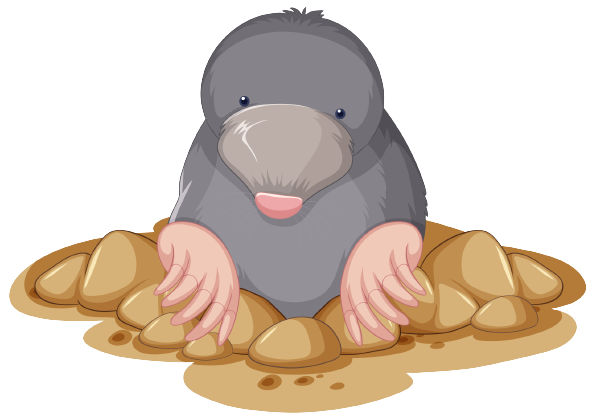
\includegraphics[width=.6\textwidth]{./media/image3c.png}
\end{center}

\fonte{José Carlos Aragão. \emph{No palco, todo mundo vira bicho:} novas
fábulas de Esopo adaptadas para teatro. São Paulo: Planeta do Brasil,
2007. p. 39.}
\end{myquote}

Textos como esse são semelhantes:

\begin{escolha}[itemsep=-5pt]
\item ao roteiro de cinema.

\item à entrevista.

\item à reportagem.

\item ao jornal de rádio.
\end{escolha}

\num{3} Leia um trecho do conto ``Água da vida''.

\begin{myquote}
\textbf{Água da vida} \medskip

Houve, uma vez, um rei muito poderoso, que vivia feliz e tranquilo em
seu reino. Um belo dia, adoeceu gravemente e ninguém tinha esperanças de
que escapasse. Ele tinha três filhos {[}...{]}.

Encontravam-se eles no jardim do castelo a chorar e, de repente, viram
surgir à sua frente um velho de aspecto venerável, que indagou a causa
de tamanha tristeza. Disseram-lhe que estavam aflitos porque o pai
estava gravemente enfermo e os médicos já não tinham esperanças de o
salvar.

\begin{center}
\noindent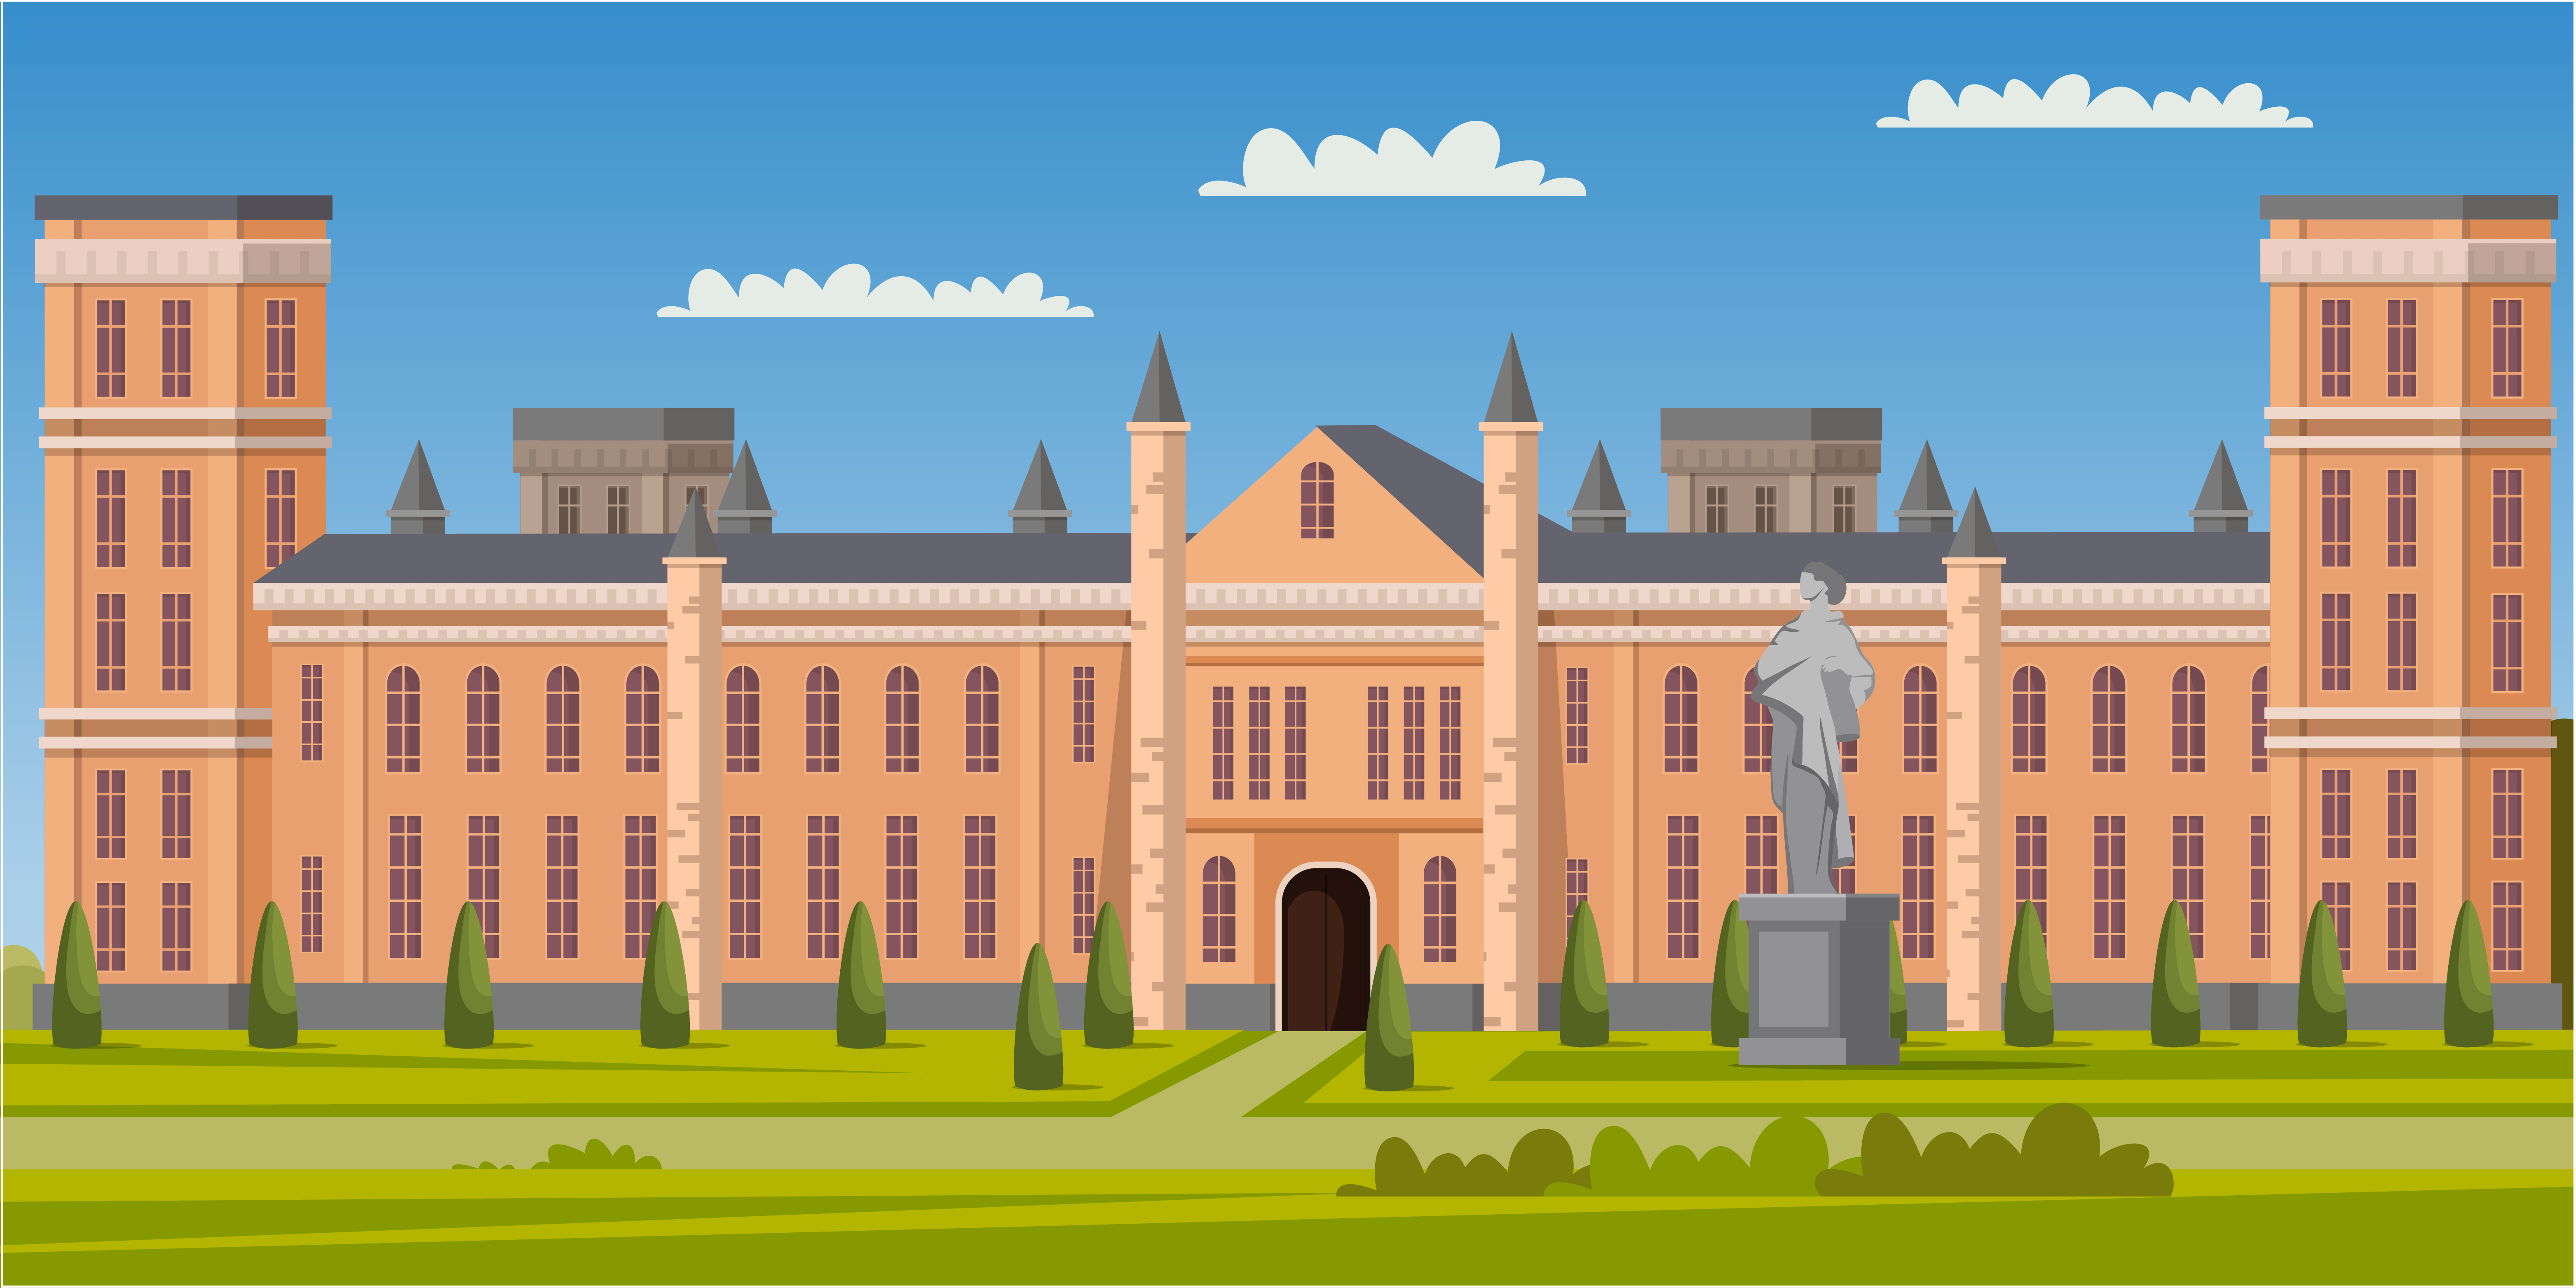
\includegraphics[width=\textwidth]{./media/image3d.jpeg}
\end{center}

O velho, então, disse-lhes:

--- Eu conheço um remédio muito eficaz, que poderá curá-lo; é a famosa
água da vida. Mas é muito difícil obtê-la. {[}...{]}

\fonte{Irmãos Grimm. A água da vida. Disponível em:
\emph{https://www.grimmstories.com/pt/grimm\_contos/a\_agua\_da\_vida}. Acesso
em: 16 fev. 2023.}
\end{myquote}

Em relação ao narrador do conto, ele

\begin{escolha}[itemsep=-5pt]
\item participa da história.

\item não participa da história.

\item é personagem da história.

\item realiza ações da história.
\end{escolha}

\chapter{Sinais de pontuação}
\markboth{Módulo 3}{}

%\coment{Neste módulo, espera-se que os alunos identifiquem os sinais de pontuação e analisem os efeitos de sentido decorrentes do uso da pontuação em diversos tipos de textos.}

\section*{Habilidades do SAEB}

\begin{itemize}
  \item Analisar elementos constitutivos de gêneros textuais diversos.
  \item Reconhecer os usos da pontuação.
  \item Analisar os efeitos de sentido decorrentes do uso da pontuação.
\end{itemize}

\subsection{Habilidades da BNCC}

\begin{itemize}
  \item EF03LP07, EF03LP16.
\end{itemize}

%\conteudo{
%\textbf{https://pixabay.com/pt/illustrations/sinais-de-pontua\%c3\%a7\%c3\%a3o-palavra-l\%c3\%adngua-2999583/}

%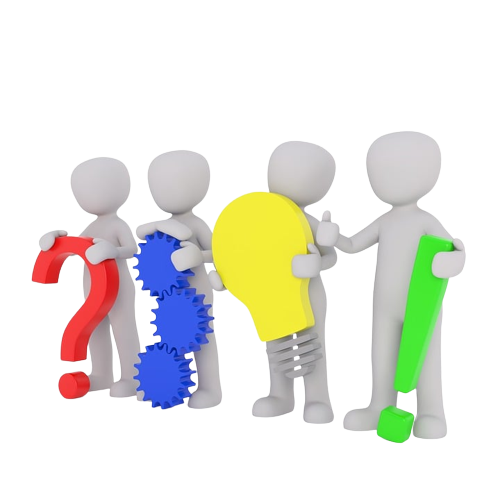
\includegraphics[width=3.41667in,height=3.41667in]{./media/image4.png}

\conteudo{
Observe, a seguir, os sinais de pontuação. Eles servem para organizar 
um texto escrito e auxiliam na construção de sentidos pretendida por 
quem escreve.

\begin{center}
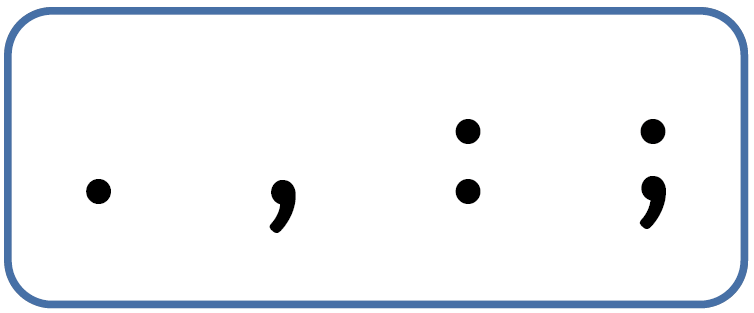
\includegraphics[width=.4\textwidth]{./media/image4b.png}
\end{center} 

Para entender melhor esse assunto, leia em voz alta um trecho do conto ``O
rouxinol do imperador'', atentando-se à pontuação: faça pausas curtas, quando 
houver vírgulas, e prolongue a respiração ao encontrar um ponto.
}

\pagebreak
\begin{myquote}
\textbf{O rouxinol do imperador}

{[}...{]} Um dia, um {[}livro{]} chegou às mãos do imperador. O soberano o leu e
ficou, ao mesmo tempo, surpreso e enfurecido. Mandou logo chamar o
primeiro-ministro.

--- Incrível! No bosque que faz divisa com os jardins imperiais, vive um
rouxinol cujo canto é incomparável, e eu o desconheço! Tive que ler um
livro estrangeiro para aprender que a maior maravilha de meu país é um
pássaro de voz de ouro, e não este meu soberbo palácio! Diga-me, por que
não fui informado?

\begin{center}
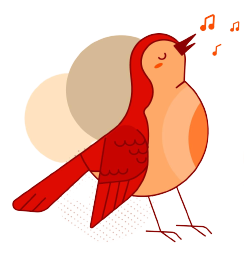
\includegraphics[width=.6\textwidth]{./media/image4a.png}
\end{center}

--- Eu também ignorava o fato, meu senhor --- respondeu o
primeiro-ministro, assustado com a ira do imperador. --- Mas vou
descobri-lo.

--- E que seja muito breve. Nesta noite mesmo o rouxinol deverá cantar
somente para mim. {[}...{]}

\fonte{Hans Christian Andersen. O rouxinol do imperador. Disponível em:
\emph{http://www.dominiopublico.gov.br/download/texto/me000589.pdf}.
Acesso em: 16 fev. 2023.}
\end{myquote}

\pagebreak

\conteudo{O texto apresenta diferentes sinais de pontuação. Entre eles, estão o ponto (\textbf{.}),
o travessão (\textbf{---}), o ponto de exclamação (\textbf{!}) e o ponto de
interrogação (\textbf{?}). Perceba que o travessão indica a fala das
personagens; e esses diálogos fazem com que o leitor tenha a sensação de
assistir à conversa, como se acontecesse no momento em que lê. O ponto
de exclamação intensifica a mensagem. O ponto de
interrogação indica pergunta. O ponto marca o fim de uma frase.}

\section*{Atividades}

\num{1} Leia o texto a seguir. Depois, responda aos itens propostos.

%Inserir imagem ao lado do texto: https://pixabay.com/pt/vectors/lobo-bonitinho-animal-personagem-1454420/

\begin{myquote}
\textbf{O lobo e o cordeiro}

\begin{wrapfigure}{l}{.5\textwidth}
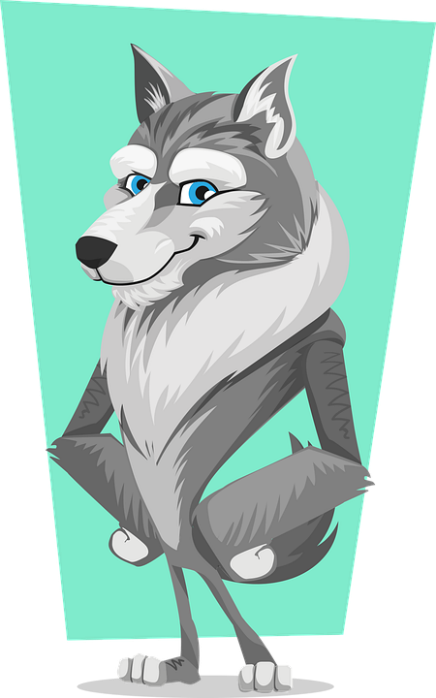
\includegraphics[width=1.97917in,height=3.16667in]{./media/image5.png}
\end{wrapfigure}

Um lobo estava bebendo água num riacho. Um cordeirinho chegou e também
começou a beber, um pouco mais para baixo.

O lobo arreganhou os dentes e disse ao cordeiro:

--- Como é que você tem a ousadia de vir sujar a água que estou bebendo?

--- Como sujar? --- Respondeu o cordeiro. --- A água corre daí para cá,
logo eu não posso estar sujando sua água.

--- Não me responda! --- Tornou o lobo furioso.

--- Há seis meses seu pai me fez a mesma coisa!

--- Há seis meses eu nem tinha nascido. Como é que eu posso ter culpa
disso? --- Respondeu o cordeiro.

--- Mas você estragou todo o meu pasto --- Replicou o lobo.

--- Como é que posso ter estragado seu pasto, se nem dentes eu tenho?

O lobo, não tendo mais como culpar o cordeiro, não disse mais nada:
pulou sobre ele e o devorou.

\fonte{O lobo e o cordeiro. Disponível em:
\emph{http://www.dominiopublico.gov.br/download/texto/me000589.pdf}.
Acesso em: 16 fev. 2023.}
\end{myquote}

\begin{escolha}[itemsep=-5pt]
\item Quem são os personagens do texto?
\reduline{O lobo e o cordeiro.\hfill}

\item Onde a história acontece?
\reduline{Na beira de um riacho.\hfill}

\item Qual é o assunto tratado no texto?
\reduline{Trata-se da história de um lobo que queria encontrar motivos para matar um cordeiro.\hfill}
\end{escolha}

\num{2} Releia o trecho do texto a seguir e responda aos itens.

\begin{myquote}
\textit{ }

--- Não me responda! --- Tornou o lobo furioso.

--- Há seis meses seu pai me fez a mesma coisa!

--- Há seis meses eu nem tinha nascido, como é que eu posso ter culpa disso? --- respondeu o cordeiro.
\end{myquote}

\begin{escolha}[itemsep=-5pt]
\item Que sinais de pontuação aparecem em final de frase nesse trecho?
\reduline{Ponto final, ponto de exclamação e ponto de interrogação.\hfill}

%\item Explique a função de cada um desses sinais de pontuação. Usa-se o
%ponto final quando se quer finalizar uma frase ou um período. Utiliza-se
%o ponto de exclamação para enfatizar o que foi dito. Usa-se o ponto de
%interrogação quando se formula uma pergunta.
%\reduline{Explique aos alunos que frases terminadas com ponto final denominam-se \textbf{frases} \textbf{declarativas}; as terminadas com ponto de interrogação denominam-se \textbf{frases} \textbf{interrogativas}; as que terminam com ponto de exclamação denominam-se \textbf{frases} \textbf{exclamativas}.\hfill}

\item Que função tem o travessão no início do texto?
\reduline{O travessão no início do texto indica a fala da personagem.\hfill}

\item Que função tem o segundo travessão no texto?
\reduline{A segunda ocorrência do travessão marca o fim da fala do personagem e o início da fala do narrador.\hfill}
\end{escolha}

\num{3} Releia o fim da história.

\begin{myquote}
O lobo, não tendo mais como culpar o cordeiro, não disse mais nada:
pulou sobre ele e o devorou.
\end{myquote}

O que ponto indica no trecho destacado?

\reduline{O ponto indica o final do trecho em destaque.\hfill}

\num{} Leia o trecho de um tradicional conto de fada, para responder 
do item 4 ao item 10. 

%\textbf{\textless{}Arte: colocar cor nos sinais destacados com grifa-texto.\textgreater{}}

%Inserir imagem ao lado do texto: https://www.istockphoto.com/br/vetor/branca-de-neve-ilustra\%C3\%A7\%C3\%A3o-vetorial-gm521993146-91504715?utm\_source=pixabay\&utm\_medium=affiliate\&utm\_campaign=SRP\_illustration\_sponsored\&utm\_content=https\%3A\%2F\%2Fpixabay.com\%2Fpt\%2Fillustrations\%2Fsearch\%2Fbranca\%2520de\%2520neve\%2F\&utm\_term=branca+de+neve

\enlargethispage{3\baselineskip}
\begin{myquote}
\textbf{Branca de Neve}\medskip 

{[}...{]} Alguns meses depois, o desejo da rainha foi atendido. Ela deu à luz uma
menina de cabelos bem pretos, pele branca e face rosada. O nome dado à
princesinha foi Branca de Neve.

\begin{wrapfigure}{l}{.3\textwidth}
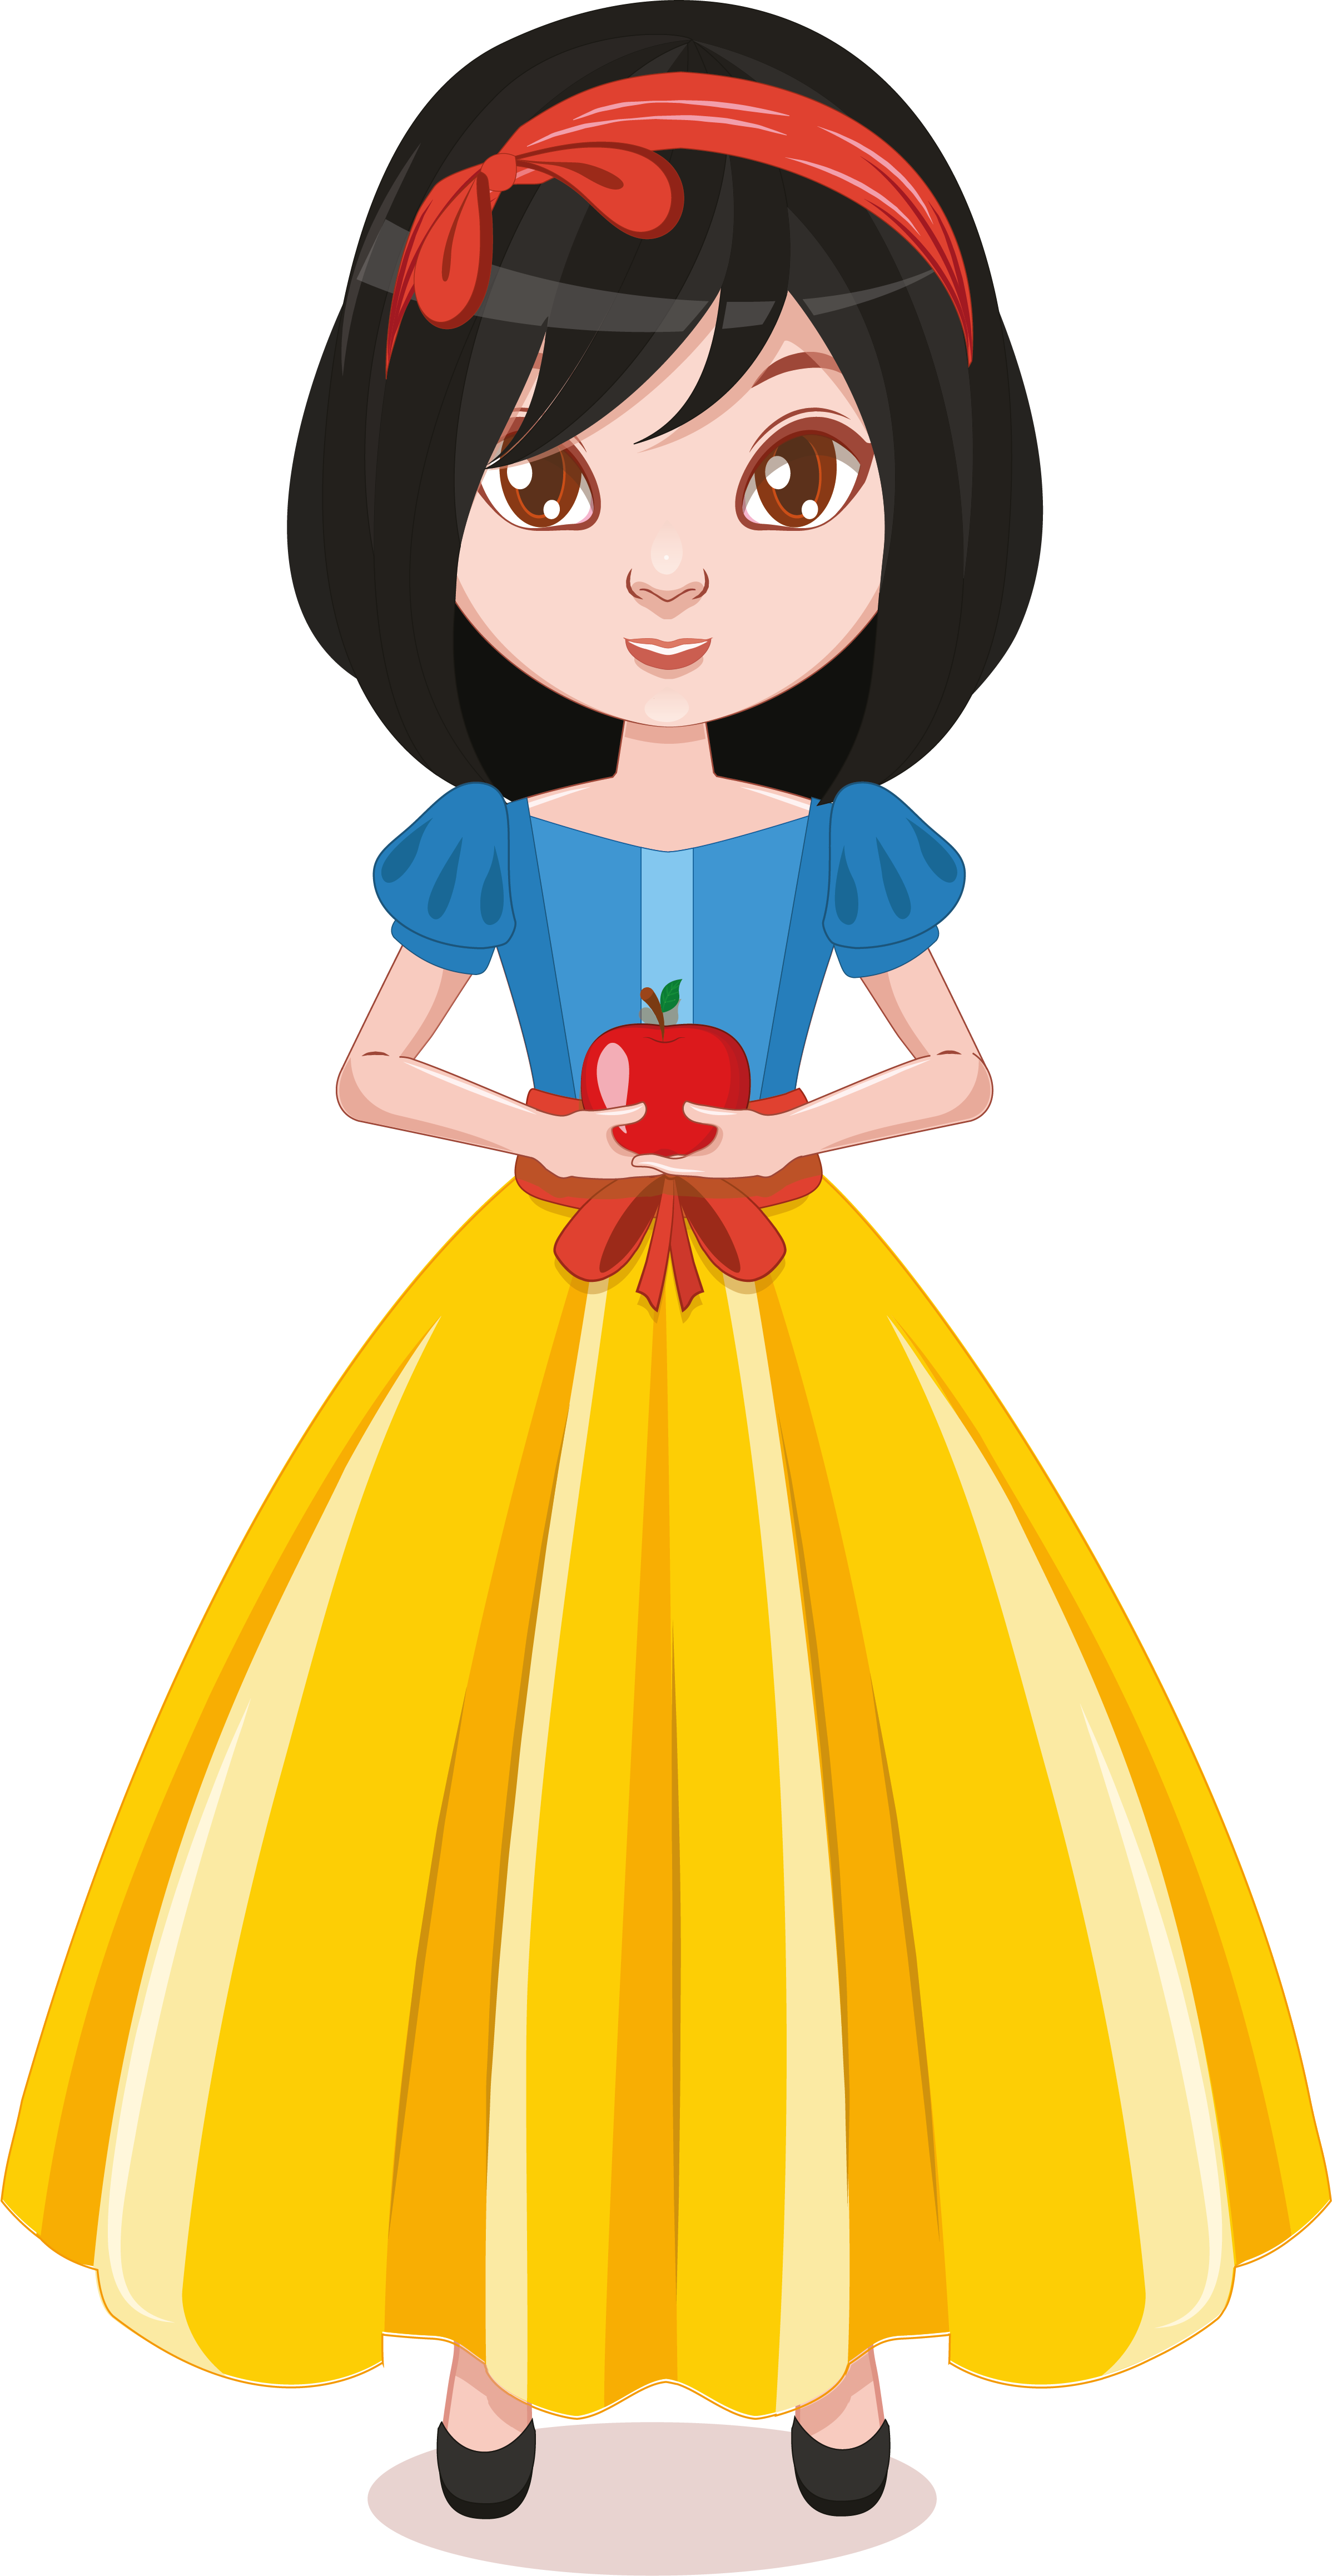
\includegraphics[width=1.5in,height=2in]{./media/image6.png}
\end{wrapfigure}

Mas, quando nasceu a menina, a rainha morreu. Passado um ano, o rei se
casou novamente. Sua esposa era lindíssima, mas muito vaidosa, invejosa
e cruel\textcolor{red}{\textbf{.}}

Um feiticeiro lhe dera um espelho mágico, ao qual todos os dias ela
perguntava, com vaidade\textcolor{red}{\textbf{:}}

\textcolor{red}{\textbf{---}} Espelho, espelho meu, diga-me se há no mundo mulher mais bela do que
eu.

E o espelho respondia:

--- Em todo o mundo, minha querida rainha, não existe beleza maior. {[}...{]}

\fonte{Branca de Neve. Disponível em:
\emph{http://www.dominiopublico.gov.br/download/texto/me000589.pdf}. Acesso em:
16 fev. 2023.}
\end{myquote}
\pagebreak

\num{4} O que a esposa do rei perguntava todos os dias ao espelho?

\reduline{Ela perguntava se no mundo havia mulher mais bela do que ela.\hfill}
\linhas{1}

\num{5} Se a frase ``--- Espelho, espelho meu, diga-me se há no mundo mulher
mais bela do que eu.'' fosse uma pergunta, como ela seria escrita?
Marque a alternativa correta.

\reduline{ --- Espelho, espelho meu, há no mundo mulher mais bela do que eu?\hfill}

\num{6} Qual o nome dado ao sinal de pontuação destacado em vermelho no início do texto? 

\reduline{Travessão.\hfill}

\num{7} Qual o nome dado ao sinal de pontuação destacado em vermelho no final do texto? 

\reduline{Ponto.\hfill}

\num{8} Qual sinal indica que o personagem vai falar?

\reduline{Os dois-pontos.\hfill}

\num{9} Complete a frase com a pontuação adequada:

\begin{escolha}[itemsep=-5pt]
\item Que dia lindo
\reduline{Ponto de exclamação.\hfill}

\item Que horas são
\reduline{Ponto de interrogação.\hfill}

\item Acrescente 200 g de manteiga
\reduline{Ponto.\hfill}

\item Então, o cordeiro respondeu
\reduline{Dois-pontos.\hfill}
\end{escolha}

\num{10} Crie uma frase de sua autoria usando a pontuação adequada.

\reduline{Auxilie os alunos na atividade, lembrando-os da função do ponto, do ponto de exclamação, ponto de interrogação, dois-pontos e travessão.\hfill}

\pagebreak
\section*{Treino}

\num{1} Leia o anúncio da campanha de vacinação contra o sarampo.

%https://www.pmna.ms.gov.br/noticias/saude/sarampo-filhos-de-seis-meses-a-menores-de-um-ano-de-idade-que-irao-viajar-para-municipios-em-situacao-de-surto-ativo-devem-vacinar

\begin{center}

\includegraphics[width=\textwidth]{./media/image7.jpeg}
\end{center}

A frase do anúncio é:

\begin{escolha}[itemsep=-5pt]
\item
  declarativa.
\item
  exclamativa.
\item
  interrogativa.
\item
  negativa.
\end{escolha}

\num{2} Leia o trecho extraído da história ``O gato de botas''.

\begin{myquote}
\textbf{O gato de botas}

Um lavrador trabalhara muito, durante a vida toda, ganhando sempre o
suficiente para o sustento da família. Quando faleceu, deixou sua
herança para os filhos: um sítio, um burrinho e um gato.

\begin{center}
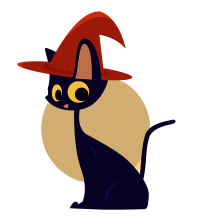
\includegraphics[width=.4\textwidth]{./media/image7a.png}
\end{center}

Ao filho mais velho coube o sítio; ao segundo, o burrinho; e o caçula
ficou com o gato. Este último, nada satisfeito com o que lhe coubera,
resmungou: ``Meus irmãos sobreviverão honestamente. Mas e eu? O que vou
fazer? Talvez possa jantar o gato e com o couro fazer um tamborim. Mas e
depois?''

O gato logo endireitou as orelhas, querendo ouvir melhor um assunto de
tamanho interesse. Então, percebendo que precisava agir, foi dizendo:

--- Não se desespere, patrãozinho, pois eu tenho um plano. Consiga-me um
par de botas e um saco de pano, e deixe o resto comigo. {[}...{]}

\fonte{O gato de botas. Disponível em:
\emph{http://www.dominiopublico.gov.br/download/texto/me000589.pdf}.
Acesso em: 17 fev. 2023.}
\end{myquote}

Que sinal de pontuação indica diálogo no trecho?

\begin{escolha}
\item
  A vírgula.
\item
  O ponto final.
\item
  O travessão.
\item
  O ponto de interrogação.
\end{escolha}


\num{3} Leia o trecho de um manual.

\begin{myquote}
\textbf{Manual Aventura Científica}

{[}...{]}

\begin{enumerate}
\item Destaque as cartas.
\item Embaralhe as cartas EU QUERO SABER e deixe-as em um monte com a
face Eu Quero Saber virada para cima, no lugar marcado no tabuleiro.
\item Embaralhe as cartas A-HÁ e deixe-as em um monte, com a face A-HÁ
virada para cima, no lugar marcado no tabuleiro.
\item Deixe as peças dos quadros espalhadas ao lado do tabuleiro, com o
lado da ilustração virada para cima, ao alcance de todos os jogadores.
\item Cada jogador escolhe um peão e coloca-o no local marcado no
tabuleiro.
\end{enumerate}

{[}...{]}

\fonte{Manual Aventura Científica. Disponível em:
\emph{https://estrela.vteximg.com.br/arquivos/Manual-Aventura-Cientifica-Show-da-Luna.pdf}. Acesso em: 17 fev. 2023.}
\end{myquote}

O objetivo desse texto é

\begin{escolha}[itemsep=-5pt]
\item dar informações relacionadas à ciência.

\item mostrar as instruções relativas a um jogo.

\item convencer o leitor a jogar um jogo de aventura.

\item ajudar o leitor a solucionar problemas de um jogo.
\end{escolha}

\chapter{Argumentação}
\markboth{Módulo 4}{}


%\coment{Neste módulo, espera-se que os alunos leiam e compreendam autonomamente texto do campo da vida pública; relacionem a imagem no texto à mensagem (linguagens verbal e não verbal); relacionem a finalidade do texto às estratégias de convencimento; identifiquem a função social do texto, reconhecendo para que serve e a quem se destina; identifiquem a ideia central do texto, compreendendo-o globalmente; e infiram informações implícitas no texto.}

\section*{Habilidades do SAEB}

\begin{itemize}
  \item Analisar o uso de recursos de persuasão em textos verbais e/ou
  multimodais.
  \item Analisar os efeitos de sentido de recursos multissemióticos em
  textos que circulam em diferentes suportes.
  \item Julgar a eficácia de argumentos em textos.
\end{itemize}

\subsection{Habilidades da BNCC}

\begin{itemize}
  \item EF03LP19.
\end{itemize}

\conteudo{%\textbf{https://pixabay.com/pt/photos/paris-fran\%c3\%a7a-cidade-cidades-urbano-195327/}

\textbf{Anúncio publicitário}

Anúncio publicitário é um gênero textual que tem como finalidade divulgar uma ideia, um produto, um valor ou um conceito. 
Essa divulgação é feita para persuadir, isto é, convencer o público em relação ao que está sendo veiculado, como a comprar um produto, a realizar uma ação ou a adotar um comportamento.

Como o principal objetivo do anúncio é persuadir o leitor,
todos os elementos nele presentes são muito bem pensados para esse fim. Para atingir
seu objetivo, quem o elabora emprega elementos como
combinação de cores, disposição de elementos visuais, jogo de palavras e
imagens, por exemplo.

A linguagem normalmente é objetiva e o vocabulário utilizado é dirigido
ao público ao qual o anúncio se destina.

Os anúncios podem ser constituídos de \emph{slogans} (frases de efeito)
e apresentam também a instituição ou a marca responsável pela sua
veiculação (logomarca).

Esse gênero textual pode ser divulgado na televisão, em revistas,
jornais, \emph{outdoors}, cartazes e anúncios na internet.

\begin{center}
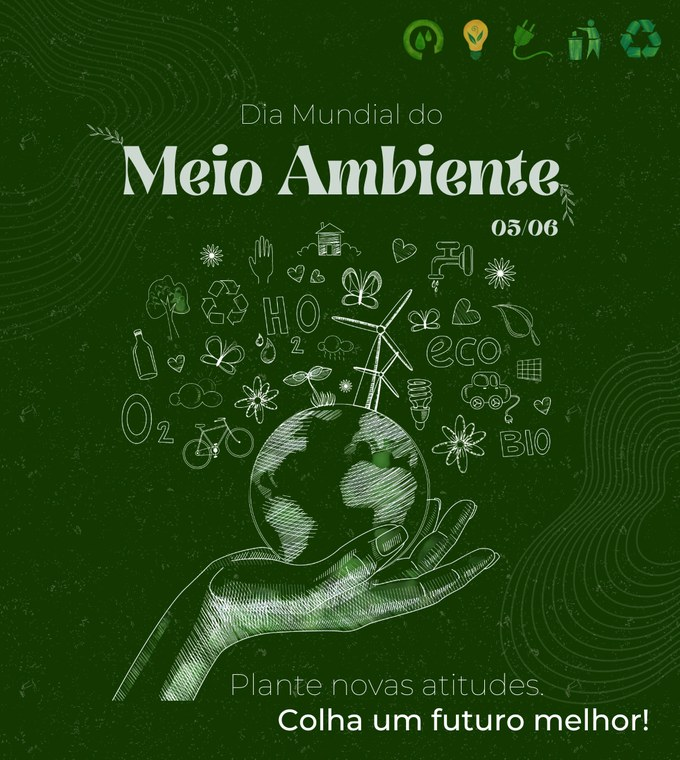
\includegraphics[width=\textwidth]{./media/image8a.jpeg}
\end{center}
}

\pagebreak
\section*{Atividades}

Observe o anúncio e resolva as atividades de 1 a 6.

%\coment{Explore com os alunos o cartaz, a imagem que o compõe e os elementos verbais. Avalie com eles os motivos da escolha do produtor ao dar ênfase a alguns elementos do texto verbal, e se esse recurso foi efetivo na divulgação do que se pretendia.}

%Paulo: Inserir ilustração 1, que será produzida.

\begin{center}
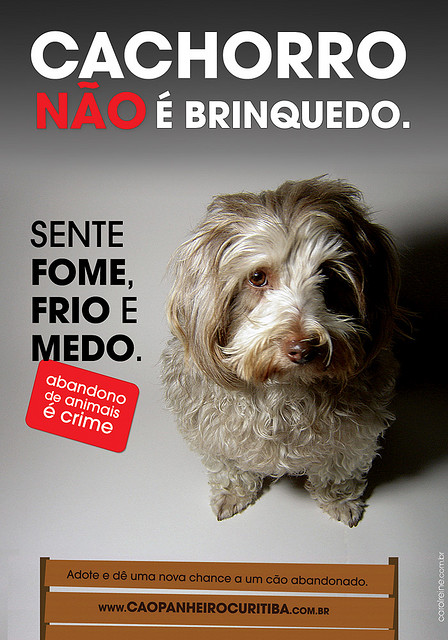
\includegraphics[width=.8\textwidth]{./media/image9.jpeg}
\end{center}

\num{1} Qual é o objetivo desse anúncio publicitário? 

\reduline{Espera-se que os alunos compreendam que um cachorro é um ser vivo. A pessoa responsável pelo animal, chamado tutor, tem a responsabilidade de garantir bem-estar e proteção.\hfill}
\linhas{2}

\num{2} Para quem esse anúncio é destinado? 

\reduline{É destinado aos tutores de animais de estimação.\hfill}
\linhas{2}

\num{3} Segundo o anúncio, por que os animais não devem ser abandonados? 

\reduline{Os animais não devem ser abandonados, porque eles sentem fome, frio e medo.\hfill}
\linhas{2}

\num{4} Como o cachorro que aparece no anúncio aparenta estar?

\reduline{O cachorro aparenta estar sozinho.}


\num{5} Em sua opinião, na frase ``Cachorro não é brinquedo'', por que a palavra \textbf{não} está com uma cor diferente do restante do texto?

\reduline{Resposta pessoal. Os alunos podem indicar que o destaque produz reforça o fato de o cachorro ser um ser vivo e não um objeto inanimado.\hfill}
\linhas{5}

\num{6} Em sua opinião, o anúncio está cumprindo sua finalidade? Justifique
sua resposta. 

\reduline{Resposta pessoal.\hfill}
\linhas{4}

\num{7} Veja a seguir mais um exemplo de cartaz de uma campanha publicitária.

%https://www.comunicaquemuda.com.br/monstros-avisam-que-lavar-as-maos-protege-de-doencas/

\begin{figure}[htpb!]
\centering
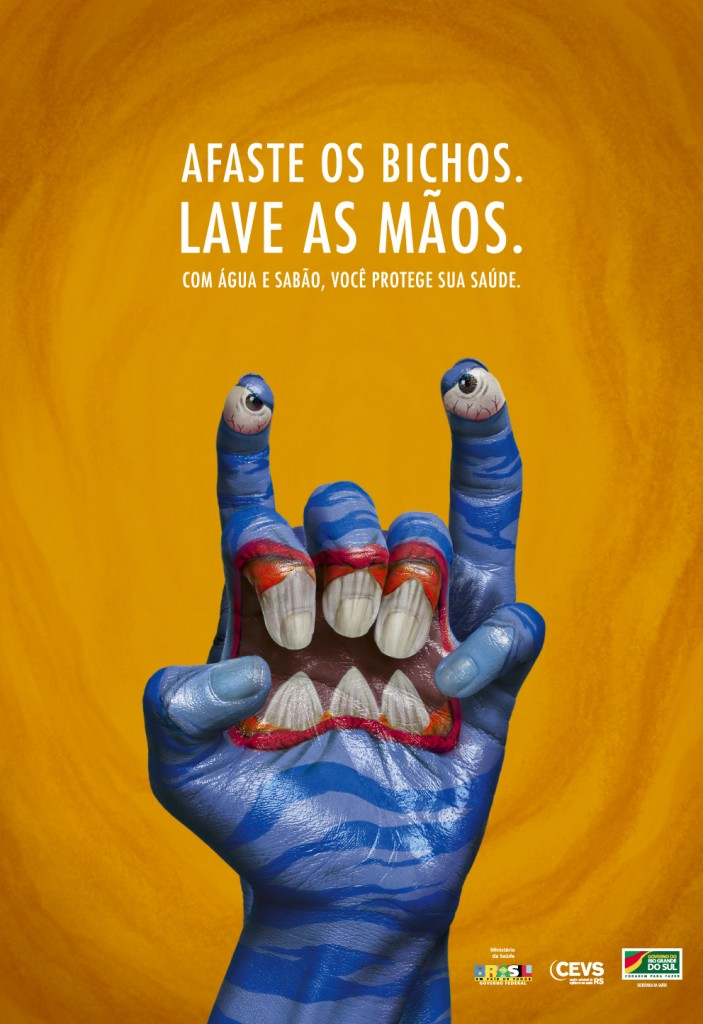
\includegraphics[width=.7\textwidth]{./media/image10.jpeg}
\end{figure}

\begin{escolha}[itemsep=-5pt]
\item Qual é o objetivo desse anúncio?
\reduline{O objetivo é orientar a população a higienizar as mãos.\hfill}

\item Você acha importante lavar as mãos? Por quê?
\reduline{Resposta pessoal. Espera-se que os alunos respondam que sim, porque é um hábito que pode impedir a propagação de micro-organismos que provocam doenças.\hfill}

\item Segundo o anúncio, o que é preciso usar para lavar as mãos e proteger a saúde?
\reduline{Água e sabão.\hfill}

\item O que a imagem da mão está representando?
\reduline{A imagem representa os micro-organismos prejudiciais à saúde que ficam nas mãos se não estão higienizadas.\hfill}
\end{escolha}

\num{8} \emph{Slogan} é uma frase curta que se destina a prender a atenção do
público. 

\begin{escolha}
\item Qual é o \emph{slogan} presente nesse anúncio?
\reduline{Afaste os bichos, lave as mãos.\hfill}
\linhas{3}

\item Quais são características que podem ser observadas no \emph{slogan} do cartaz. 
\reduline{Resposta pessoal. Os alunos podem indicar o uso de frases curta e de fácil memorização. Além disso, podem apontar a utilização de fonte de tamanhos diferentes, para chamar a atenção do leitor.\hfill}
\end{escolha}
\linhas{3}

\pagebreak
\num{9} Forme dupla com um colega, para elaborar outro \emph{slogan} para o cartaz da atividade anterior. Registre o resultado no espaço a seguir.

%\coment{Lembre os alunos de fazerem uso do imperativo nas formas verbais utilizadas como recurso para convencer o leitor.}

\begin{mdframed}[linewidth=2pt,linecolor=salmao,roundcorner=20pt]
\vspace{7cm}
\end{mdframed}

\num{10} Encontre, no caça-palavra a seguir, palavras que representam
características do texto publicitário.

\begin{myquote}
CONVENCER \hfill LOGOMARCA \hfill \textit{SLOGAN} \hfill TÍTULO \hfill
\end{myquote}

\begin{center}
\begin{tabular}{llllllllllll}
K & T & R & S & E & Y & A & E & T & E & T & F\\
P & D & A & T & S & T & O & O & E & E & U & S\\
A & T & P & I & Í & E & H & N & E & C & P & P\\
S & E & I & A & D & T & S & T & M & E & C & L\\
A & A & A & G & S & R & U & C & N & D & O & A\\
M & T & O & W & I & E & S & L & E & G & N & U\\
T & S & C & T & U & R & N & A & O & A & V & T\\
E & P & N & O & R & T & A & M & A & D & E & N\\
O & P & S & L & O & G & A & N & T & A & N & E\\
E & H & O & S & A & R & I & E & T & B & C & O\\
N & W & P & E & C & N & W & R & E & T & E & C\\
H & Y & B & A & R & Y & U & O & I & T & R & S
\end{tabular}
\end{center}
\pagebreak


% \num{10} Leia, agora, outro anúncio de campanha publicitária.

% \begin{figure}[htpb!]
% 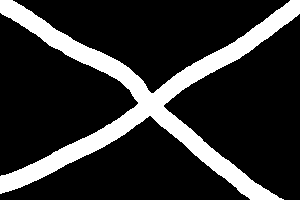
\includegraphics[width=\textwidth]{./media/confederados.png}
% \end{figure}

% %Paulo: Inseriri a ilustração 2, que será produzida.

% \begin{escolha}[itemsep=-5pt]
% \item Qual é o objetivo da campanha anunciada?
% \item\reduline{Trata-se de uma campanha para arrecadação de brinquedos e roupas.\hfill}

% \item Qual é o \textit{slogan} presente nesse anúncio?
% \item\reduline{Doe um brinquedo, ganhe um sorriso!\hfill}

% \item Onde serão coletados os brinquedos e as roupas?
% \item\reduline{Na Estação Cultural e na Secretaria de Educação.\hfill}

% \item Em sua opinião, por que doar brinquedos garante sorrisos?
% \item\reduline{Resposta pessoal. Aproveite o momento e explique aos alunos que doar é
% um ato de amor ao próximo e evita o acúmulo desnecessário. Além disso, no caso
% específico da campanha, as crianças que recebem brinquedos ficam alegres.\hfill}
% \end{escolha}


\section*{Treino}

\num{1} Leia o cartaz de conscientização.

%https://www.bombinhas.sc.gov.br/noticias/ver/2014/11/campanha-de-vacinacao-contra-sarampo-e-paralisia-infantil-inicia-neste-sabado

\begin{figure}[htpb!]
\centering
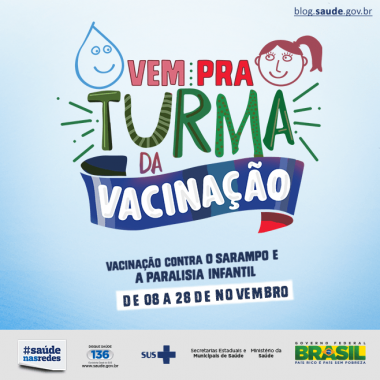
\includegraphics[width=.8\textwidth]{./media/image12.png}
\end{figure}

\fonte{Disponível em:
\emph{https://www.bombinhas.sc.gov.br/noticias/ver/2014/11/campanha-de-vacinacao-contra-sarampo-e-paralisia-infantil-inicia-neste-sabado}.
Acesso em: 18 fev. 2023.}

Compreende-se que o cartaz é parte de uma campanha sobre a importância

\begin{escolha}[itemsep=-5pt]
\item de desenhar com liberdade e criatividade.

\item de ter a própria ``turma'', ou seja, bons amigos.

\item da amizade e das brincadeiras com os amigos.

\item da vacinação contra o sarampo e a paralisia infantil.
\end{escolha}
\pagebreak

\num{2} Observe o cartaz de uma campanha.

%https://i.pinimg.com/originals/73/ce/78/73ce78802f6062e3f50dfe73c65931b4.jpg

\begin{figure}[htpb!]
\centering
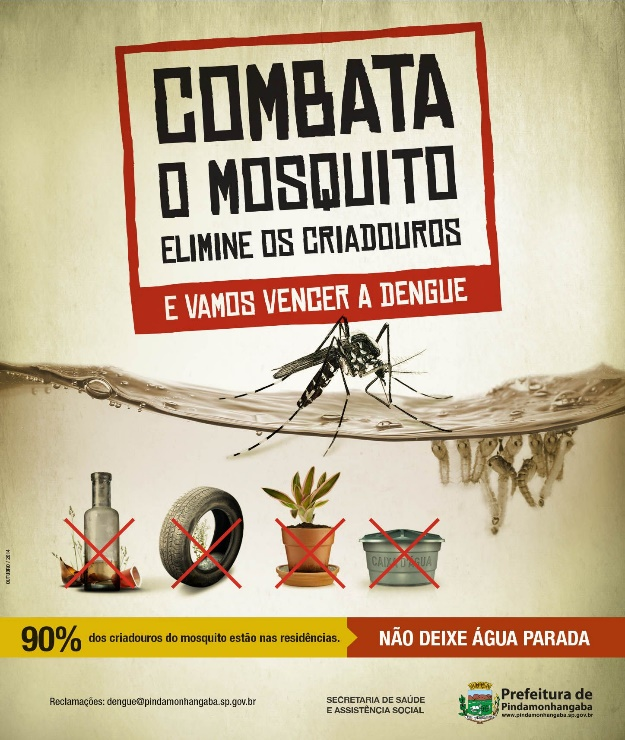
\includegraphics[width=.7\textwidth]{./media/image13.jpeg}
\end{figure}

Uma análise correta sobre elemento do cartaz é que

\begin{escolha}[itemsep=-5pt]
\item a presença da água reforça a ideia de que é preciso aguar as plantas com regularidade.

\item o sinal de corte sobre determinadas imagens aponta para aquilo que deve ser evitado.

\item a representação do mosquito não está relacionada ao texto principal do anúncio.

\item a imagem das larvas refere-se à necessidade de manter vivos os mosquitos na natureza.
\end{escolha}
\pagebreak

\num{3} Analise este cartaz.

%https://vitalvereador.wordpress.com/2012/01/29/campanha-vamos-tirar-o-planeta-do-sufoco/

\begin{figure}[htpb!]
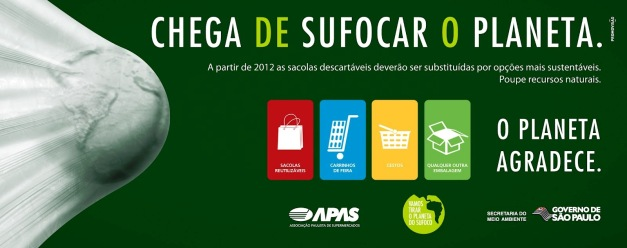
\includegraphics[width=\textwidth]{./media/image14.jpeg}
\end{figure}

\fonte{Disponível em:
\emph{https://vitalvereador.wordpress.com/2012/01/29/campanha-vamos-tirar-o-planeta-do-sufoco/}.
Acesso em: 18 fev. 2023.}

Com esse cartaz, o objetivo pretendido

\begin{escolha}[itemsep=-5pt]
\item não pode ser alcançado.

\item pode ser alcançado, mas não está claro o que o motiva.

\item está alcançado na medida em que fica clara a ideia defendida.

\item seria alcançado se o texto fosse dirigido diretamenteo ao leitor.
\end{escolha}

\chapter{O texto em versos}
\markboth{Módulo 5}{}

%\coment{Neste módulo, espera-se que os alunos localizem informações explícitas no poema; identifiquem a função social do texto, reconhecendo a sua função, onde circula, quem o produziu e a quem se destina; reconheçam características do poema, como estrofes e versos, rimas nos versos; notem a relação entre textos; reconheçam o sentido figurado de palavras e expressões utilizadas no poema; infiram o sentido de palavras, com base no contexto de trecho de texto.}

\section*{Habilidades do SAEB}

\begin{itemize}
  \item Reconhecer diferentes modos de organização composicional de
  textos em versos.
  \item Analisar a construção de sentidos de textos em versos com base
  em seus elementos constitutivos.
\end{itemize}

\subsection{Habilidades da BNCC}

\begin{itemize}
\item EF35LP16, EF03LP26, EF35LP27, EF35LP31.
\end{itemize}

\conteudo{
%\href{https://www.istockphoto.com/br/vetor/escritora-cria-poesia-com-pena-no-papel-gm1346126990-423980947?utm_source=pixabay\&utm_medium=affiliate\&utm_campaign=SRP_vector_sponsored\&utm_content=https\%3A\%2F\%2Fpixabay.com\%2Fpt\%2Fvectors\%2Fsearch\%2Fpoema\%2F\%3Fmanual_search\%3D1\&utm_term=poema}{https://www.istockphoto.com/br/vetor/escritora-cria-poesia-com-pena-no-papel-gm1346126990-423980947?utm\_source=pixabay\&utm\_medium=affiliate\&utm\_campaign=SRP\_vector\_sponsored\&utm\_content=https\%3A\%2F\%2Fpixabay.com\%2Fpt\%2Fvectors\%2Fsearch\%2Fpoema\%2F\%3Fmanual\_search\%3D1\&utm\_term=poema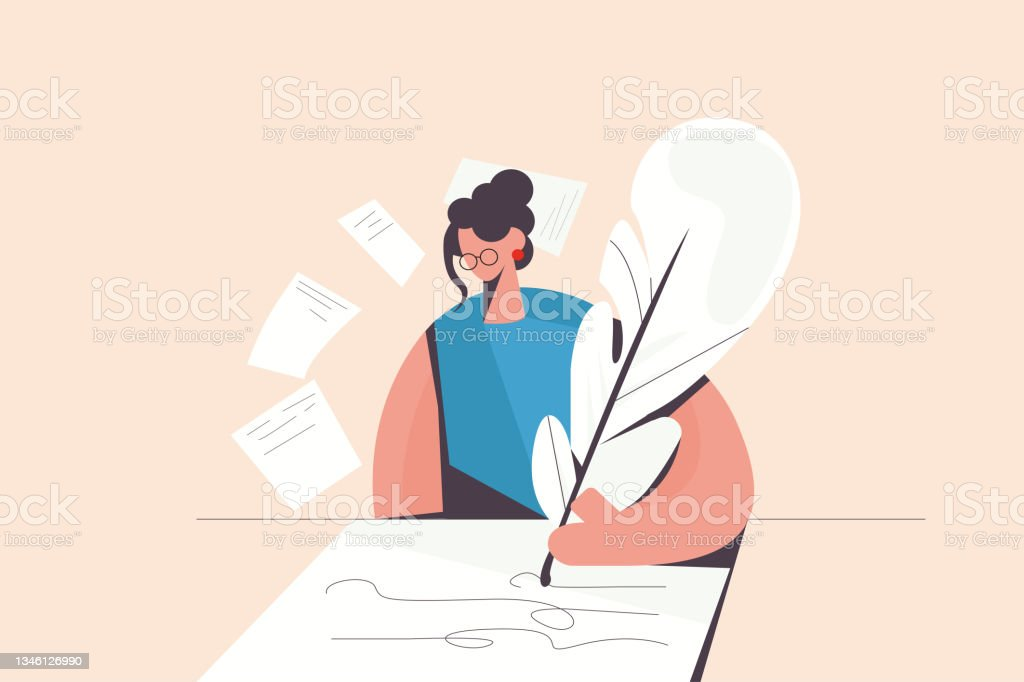
\includegraphics[width=4.80139in,height=3.19792in]{./media/image15.jpeg}}

O \textbf{poema} é o texto organizado em versos. 
Sua principal característica é explorar a linguagem de modo
diferenciado, isto é, utiliza a sonoridade das palavras (pode apresentar rima,
repetição de sons e ritmo) e utiliza termos e expressões no sentido
figurado -- com significado diferente daquele que normalmente apresenta.

A cada uma das linhas de um poema damos o nome de \textbf{verso}. Alguns poemas
podem ser organizados em conjuntos de versos separados por uma linha em
branco. Esses conjuntos de versos denominam-se \textbf{estrofes}. Nas
estrofes, pode ou não haver rimas entre os versos que as compõem.

Em um texto poético, é necessário fazer a distinção entre o poeta, ou
seja, o escritor, do \textbf{eu que fala no texto}. Em texto narrativos, por
exemplo, quem dá a voz denomina-se narrador, mas, nos poemas, a voz
é a do \textbf{eu lírico}, que pode expressar
sentimentos, ideias e emoções que permitem envolver o leitor e
despertar nele as mais diferentes sensações.

Além disso, a escolha
cuidadosa das palavras e a forma como são organizadas no texto conferem
beleza ao poema e também são responsáveis por atrair o interesse dos
leitores.

O poema pode apresentar as mais variadas estruturas. A mais tradicional tem
estrutura na vertical, isto é, um verso embaixo do outro. Os versos
poderão ser agrupados em estrofes, e as estrofes são, geralmente,
separadas por uma linha em branco.

É o poeta quem escolhe o título (se houver) e o tamanho do poema. É bom lembrar que
as escolhas realizadas pelo
poeta levam em consideração que, normalmente, o texto poético procura
sensibilizar o leitor, provocando sentimentos e emoções no momento da
leitura.

Na elaboração do texto, o poeta pode utilizar muitos recursos poéticos,
como rima, recursos visuais e sonoros, imagens poéticas ou
onomatopeias, por exemplo.
}

\section*{Atividades}

Leia o poema e resolva as atividades de 1 a 7.

%Inserir imagem do relógio ao lado do poema. https://www.pexels.com/pt-br/foto/relogio-analogico-preto-e-amarelo-3283142/

%\begin{figure}[htpb!]
%\centering
%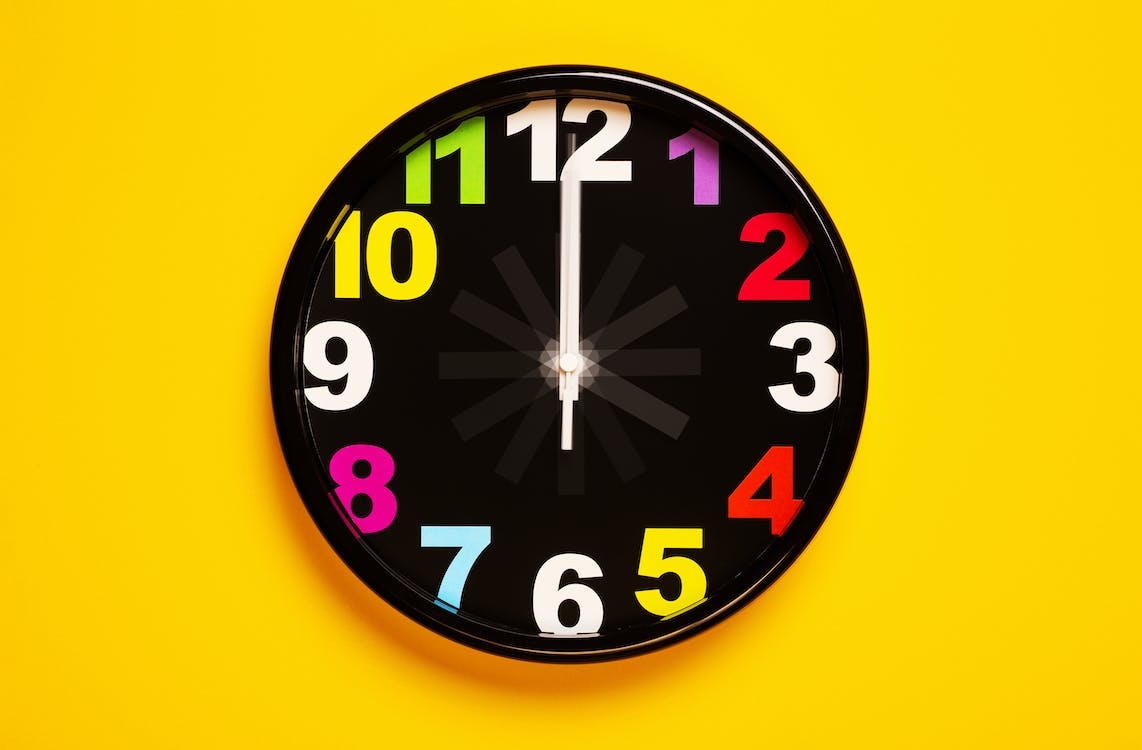
\includegraphics[width=.8\textwidth]{./media/image16.jpeg}
%\end{figure}

\begin{myquote}
\begin{verse}
\textbf{O relógio}

Preso à parede, sozinho lá,\\
Alvo dos olhos de toda gente,\\
Minutos e horas, eternamente,\\
Alma do tempo, batendo está.

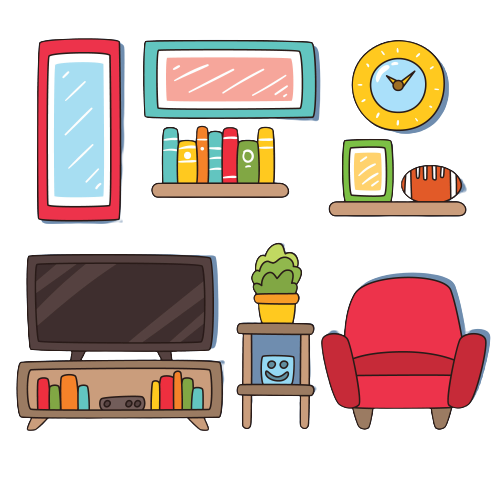
\includegraphics[width=.9\textwidth]{./media/image14a.png}

Na intimidade de todo lar\\
Se as alegrias são verdadeiras,\\
As horas correm, voam ligeiras\\
Para a ventura não demorar.

Gelam os risos, e quando enfim\\
Dor ou tristeza nos olhos chora,\\
Calmo, o relógio para e demora,\\
A hora parece que não tem fim.
\end{verse}

\fonte{Francisca Julia e Julio da Silva. \textbf{Alma infantil:} versos para
uso das escolas. São Paulo/Rio de Janeiro: Editora Livraria Magalhães,
1912. p. 25-26.}

\begin{small}
\textbf{Vocabulário:} \textit{ligeiras}: rápidas, velozes; \textit{ventura:} felicidade.
\end{small}
\end{myquote}

\num{1} Qual é o título do poema?

\reduline{O título do poema é ``O relógio''.\hfill}
\linhas{2}

\num{2} Quem escreveu o poema?

\reduline{Francisca Julia e Julio da Silva.\hfill}
\linhas{2}

\num{3} Em que livro esse poema foi publicado?

\reduline{O livro em que o poema foi publicado intitula-se \textit{Alma infantil}.\hfill}
\linhas{2}

\num{4} Segundo o poema, como as horas passam se as alegrias são verdadeiras?

\reduline{As horas passam rapidamente se as alegrias são verdadeiras.\hfill}
\linhas{2}

\num{5} Leia este verbete de dicionário.

\begin{myquote}
\textbf{Gelar} (ge.lar)
\textit{v.}

\begin{enumerate}
\item Esfriar(-se) muito.
Gelou o suco antes de servir.
Estava sem meias, seus pés gelaram.

\item Adquirir dura consistência pela ação do frio; congelar(-se).
O inverno gelou o lago.
As vinhas gelaram por causa do frio.]

\item Causar forte sensação de frio; resfriar [td. : O vento frio gelou -lhe o nariz.] [int. : Os quartos do hotel não tinham aquecedores, e os hóspedes gelavam.]

\item Causar ou sentir muito medo; apavorar(-se).
A terrível cena gelou a mulher.
Diante do assaltante, o homem gelou de medo.

\item Tornar (alguém) abatido, desanimado.
A censura do diretor gelou o aluno.
Gelou quando a moça desmanchou o namoro.

\item Fazer perder ou perder o calor humano ou o ardor dos sentimentos.
As decepções da vida gelam o entusiasmo.
Sentindo-se injustiçado, gelou toda a família.
Diante do desprezo do marido, seu coração gelou.

\item Forçar a interrupção ou a suspensão de; interromper(-se); suspender(-se).
A falta de verbas gelou as bolsas de pós-graduação.
Com o mau tempo, o passeio gelou.
\end{enumerate}

\fonte{Aulete digital. Disponível em: \emph{https://aulete.com.br/gelar}. Acesso em: 19 fev. 2023.}
\end{myquote}

Agora, releia uma estrofe do poema.

\begin{myquote}
\begin{verse}
Gelam os risos, e quando enfim\\
Dor ou tristeza nos olhos chora,\\
Calmo, o relógio para e demora,\\
A hora parece que não tem fim.\\

\fonte{Francisca Julia e Julio da Silva. \textbf{Alma infantil:} versos para
uso das escolas. São Paulo/Rio de Janeiro: Editora Livraria Magalhães,
1912. p. 25-26.}
%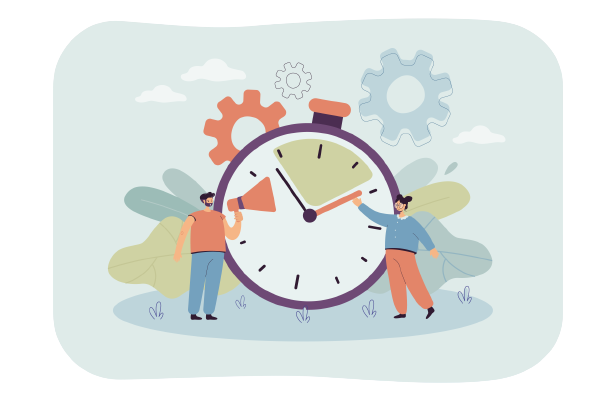
\includegraphics[width=.6\textwidth]{./media/image14b.png}
\end{verse}
\end{myquote}

\pagebreak
Em sua opinião, a palavra ``gelam'' tem o mesmo sentido que qual item do verbete? Justifique sua resposta.

\reduline{O verbo ``gelar'' foi empregado com o sentido expresso no item 7 do verbete.\hfill}
\linhas{4}

\num{6} Como é a divisão do poema em versos e estrofes?

\reduline{O poema tem um total de doze verssos, divididos igualmente em três estrofes de quatro versos.\hfill}
\linhas{3}

\num{7} Como se dão as rimas no poema?

\reduline{Os pares de palavras que rimam entre si são estes: lá/está; gente/eternamente;
lar/demorar; verdadeiras/ligeiras; enfim/fim; chora/demora.\hfill}
\linhas{4}

Leia o poema e resolva as atividades de 8 a 12.

%\coment{Promova uma leitura expressiva desse poema. Desse modo, estará desenvolvendo a fluência, identificação e apreciação de textos em versos.}

%Inserir imagem ao lado do poema:
%https://pixabay.com/pt/vectors/gato-scottish-fold-gatinho-gatinha-7753428/

\begin{myquote}
\bigskip
\begin{minipage}{.5\textwidth}
\textbf{Uma amiguinha}\bigskip


É inteligente e graciosa;\\
Mais limpa, que ela, não há:\\
Focinhito cor‑de‑rosa,\\
E chama‑se Resedá.

Muito orgulhosa e faceira,\\
Não quer saber da cozinha,\\
E, à sesta, sob a roseira,\\
Dorme um sono de rainha.

Gosta do sol, ama as flores,\\
Corre por todo o jardim,\\
E tem, no dorso, em três cores,\\
A maciez do cetim.

{[}...{]}

É toda mimos da sorte,\\
Gatinha de estimação,\\
Defende‑a, contra o mais forte,\\
Das patas vivo arranhão.

Mas é boazinha e correta;\\
Não provoca ásperos tratos;\\
Somente mostra‑se inquieta,\\
Se escuta rumor de ratos.
 
Então --- adeus, gentileza! ---\\
É toda instinto animal,\\
De um salto, atira‑se à presa...\\
E é como as outras, tal qual.
\end{minipage}
\begin{minipage}{.5\textwidth}
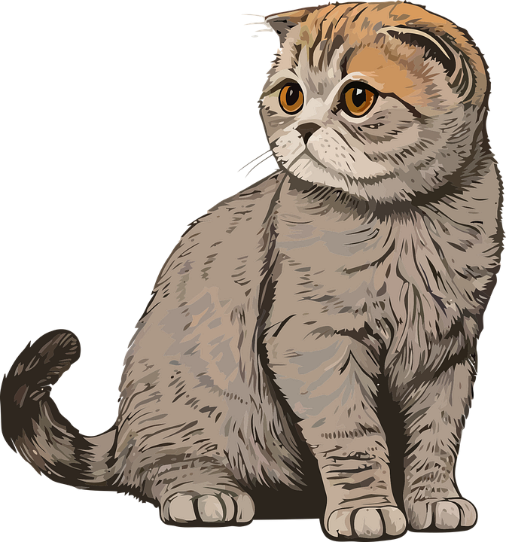
\includegraphics[width=.8\textwidth]{./media/image17.png}
\end{minipage}

\fonte{Zalina Rolim. \textbf{Livro das crianças}. Disponível em:
\emph{https://www.unicamp.br/iel/memoria/Ensaios/LiteraturaInfantil/10Zalina.htm}.
Acesso em: 11 fev. 2023.}

\begin{small}
\textbf{Vocabulário:} \textit{focinhito}: focinho; \textit{dorso}: costas; \textit{cetim}: tipo de tecido muito macio; \textit{inquieta}: agitada; \textit{rumor}: ruído.
\end{small}
\end{myquote}

\num{8} O título do texto é ``Uma amiguinha''. Quem é a amiguinha?

\reduline{A amiguinha é a gatinha Resedá.\hfill}
\linhas{3}

\num{9} Quantas estrofes e quantos versos há nesse trecho do poema?

\reduline{Nesse trecho do poema, aparecem seis estrofes, e cada uma tem quatro versos.\hfill}
\linhas{3}

\num{10} Transcreva uma rima presente no poema.

\reduline{Sugestão de resposta: rimam entre si, no poema, ``graciosa'' e ``cor-de-rosa''.\hfill}
\linhas{3}

\num{11} Quais as palavras do poema rimam com \textbf{graciosa} e \textbf{cor-de-rosa}.

\reduline{Sugestão de resposta: misteriosa e sedosa.\hfill}
\linhas{3}

% \num{12} Normalmente, representam-se os sons das rimas por letras maiúculas. Observe:

% \begin{quote}\parindent=0em
% É inteligente e graci\textbf{osa}; \textbf{A}

% Mais limpa, que ela, não h\textbf{á}: \textbf{B}

% Focinhito cor‑de‑r\textbf{osa}, \textbf{A}

% E chama‑se Resed\textbf{á}. \textbf{B}
% \end{quote}

% Isso significa que, nessa estrofe, o primeiro verso rima com o terceiro, e o segundo rima com o quarto. A letra \textbf{A}, nesse caso, representa o som repetido no final do primeiro e do terceiro verso: \textbf{osa}. Já a letra \textbf{B} represente o som repetido no final do segundo e do quarto verso: \textbf{á}.

% Agora, releia outra estrofe do poema.

% \begin{quote}
% \begin{verse}
% Mas é boazinha e correta;\\
% Não provoca ásperos tratos;\\
% Somente mostra-se inquieta,\\
% Se escuta rumor de ratos.
% \end{verse}
% \end{quote}

% Usando as letras maiúsculas C e D, represente o esquema de rimas dessa estrofe.

% \reduline{CDCD.\hfill}
% \linhas{1}


\section*{Treino}

\num{1} Leia o poema.

\begin{myquote}
\begin{verse}
\textbf{Amigos por toda a parte}

Manhã de primavera:\\
Nos ares voa um cântico festivo ---\\
Leve rumor de voz, barulho vivo,\\
Ao sol, que reverbera.

{[}...{]}

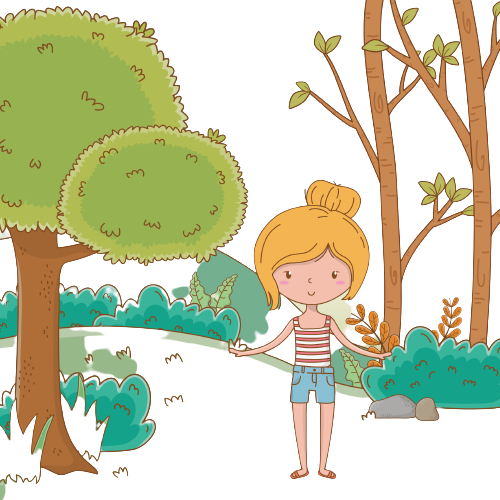
\includegraphics[width=.8\textwidth]{./media/image17a.png}
\pagebreak

Por toda a parte flores!\\
Áureas, roxas, azuis, brancas, vermelhas...\\
E, em zumbidora orquestra, andam abelhas\\
Correndo os arredores.

Gorjeiam passarinhos...\\
E Lídia vai seguindo alegremente,\\
Num bem‑estar de espírito contente,\\
Ao longo dos caminhos.

Orla, um ribeiro, a mata,\\
Alvo, entre margens de veludo eterno;\\
O gaio azul do céu de um brilho terno\\
Nas águas se retrata.

Serena paz bendita,\\
Como um perfume, estende‑se por tudo...\\
E, olhos abertos, cauteloso e mudo,\\
Fiel a cauda agita.

E os olhos tão suaves\\
De Lídia, e os doces lábios cor de rosa,\\
Riem‑se à luz do sol, fina e radiosa,\\
E ao cântico das aves.
\end{verse}


\fonte{Zalina Rolim. \textbf{Livro das crianças}. Disponível em:
\emph{https://www.unicamp.br/iel/memoria/Ensaios/LiteraturaInfantil/10Zalina.htm}.
Acesso em: 11 fev. 2023.}
\end{myquote}

Nesse trecho do poema, há

\begin{escolha}[itemsep=-5pt]
\item versos todos do mesmo tamanho.

\item estrofes com número diferentes de versos.

\item quatro versos em cada estrofe.

\item estrofes de verso único.
\end{escolha}

\pagebreak
\num{2} Leia um trecho do poma ``Infância'', de Casimiro de Abreu.

\begin{myquote}
\begin{verse}
\textbf{Infância}

\begin{center}
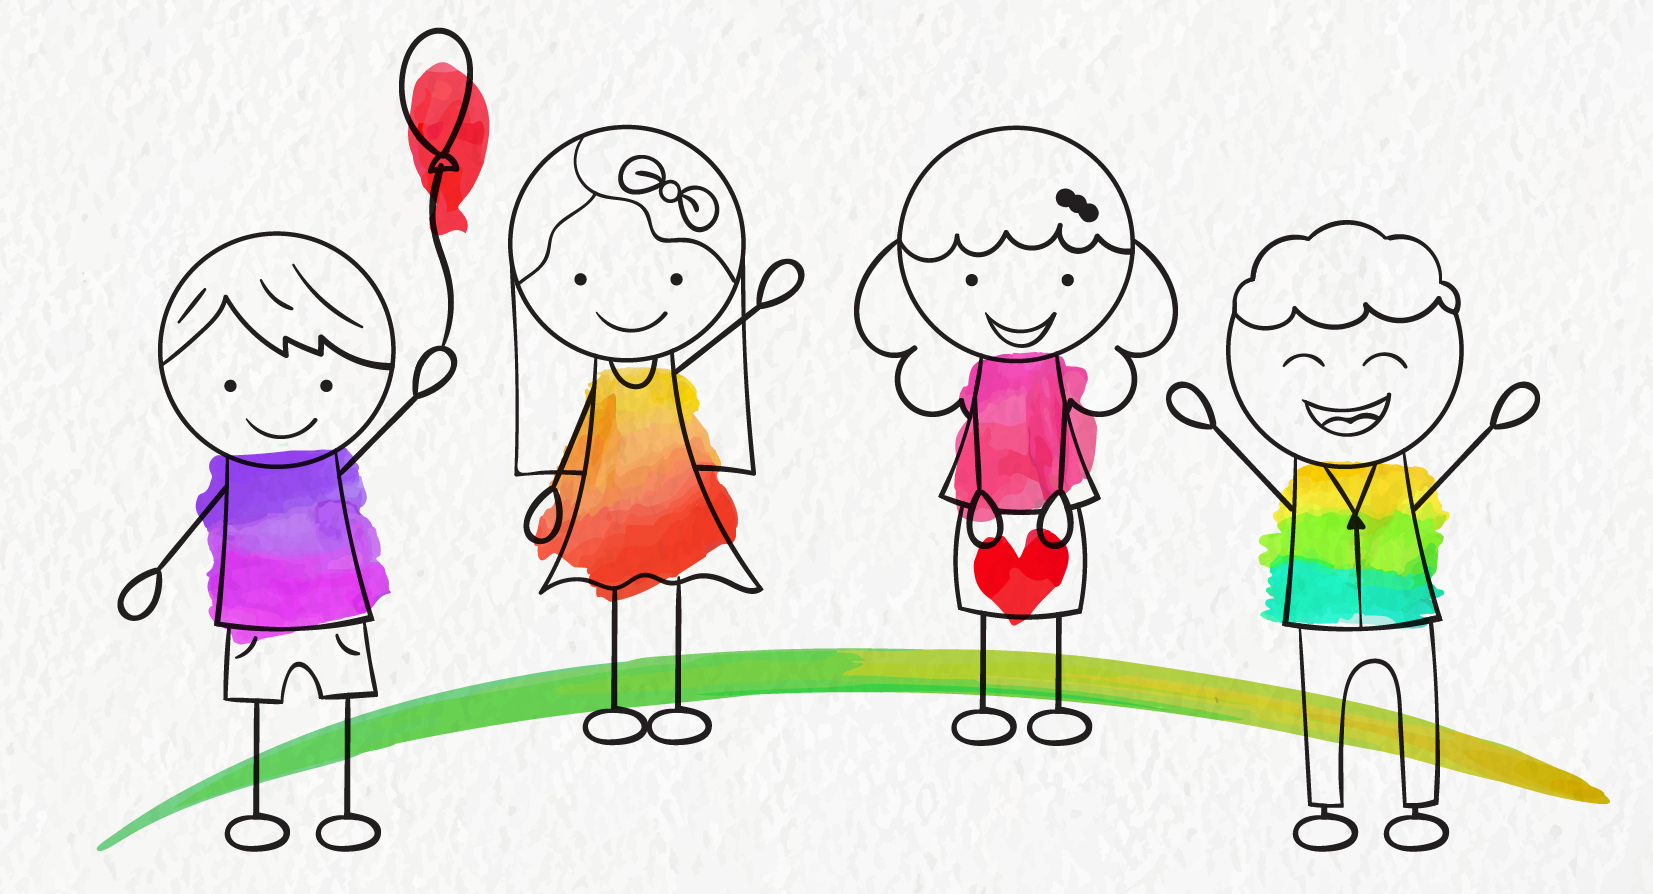
\includegraphics[width=.7\textwidth]{./media/image17b.jpeg}
\end{center}

{[}...{]}

Ó anjo da loura trança,\\
És criança,\\
A vida começa a rir.\\
--- Vive e folga descansada,\\
Descuidada\\
Das tristezas do porvir.
\end{verse}

\fonte{Casimiro de Abreu. \textbf{Infância}. Disponível em:
\emph{www.dominiopublico.gov.br/download/texto/wk000394.pdf}. Acesso em: 20
fev. 2023.}

\begin{small}
\textbf{Vocabulário:} \textit{porvir}: futuro.
\end{small}
\end{myquote}

Versos que rimam entre si, nesse trecho do poema, são

\begin{escolha}[itemsep=-5pt]
\item ``Ó anjo da loura trança'' e ``És criança''.

\item ``A vida começa a rir'' e ``Vive e folga descansada''.

\item ``Descuidada'' e ``Das tristezas do porvir''.

\item ``Ó anjo da loura trança'' e ``Vive e folga descansada''.
\end{escolha}

\num{3} Leia o poema.

\begin{myquote}
\begin{verse}
\textbf{O meu retrato}

Aquele retrato lá:\\
O corpo, as pernas, o braço,\\
Sou eu mesmo traço a traço,\\
Tão parecido ele está.

Acham bonito? Talvez...\\
O nariz é um pouco chato...\\
Mas, que importa? É o meu retrato;\\
Foi o vovô quem o fez.

{[}...{]}
\end{verse}

\fonte{Francisca Julia e Julio da Silva. \textbf{Alma infantil:} versos para uso das escolas.
Disponível em: \emph{https://digital.bbm.usp.br/bitstream/bbm/4556/1/033579\_COMPLETO.pdf}.
Acesso em: 17 abr. 2023.}
\end{myquote}

A inversão das palavras que ocorre no último verso da primeira estrofe

\begin{escolha}[itemsep=-5pt]
\item dificulta a compreensão do poema, pois cria uma incoerência.

\item enfatiza o sentido do verbo e cria uma rima com o primeiro verso.

\item gera um diferencial no poema com algo que não é típico de textos como esse.

\item é do mesmo tipo que a inversão que ocorre no último verso da segunda estrofe.
\end{escolha}

\chapter{Discurso direto e discurso indireto}
\markboth{Módulo 6}{}

\section*{Habilidade do SAEB}

\begin{itemize}
  \item Identificar as variedades linguísticas em textos.
\end{itemize}

\subsection{Habilidades da BNCC}

\begin{itemize}
  \item EF35LP22, EF35LP30.
\end{itemize}

\conteudo{
%https://pixabay.com/pt/vectors/falar-pessoas-conversa\%c3\%a7\%c3\%a3o-amigo-7647863/

O \textbf{discurso direto} é a transcrição fiel da fala de uma personagem na
narração sem a intervenção do narrador. 
Na escrita, as marcas do discurso direto podem ser: dois-pontos (\textbf{:}), 
aspas (\textbf{``''}) e travessão (\textbf{---}). 

Ele é usado para dar voz às personagens, propiciando ao leitor 
notar diferentes reações diante dos acontecimentos
que estão sendo narrados. Ele torna a
narração mais dinâmica e atraente para o leitor.

Normalmente, o discurso direto é antecidido por verbos, como falar,
dizer, comentar, perguntar, responder, observar, murmurar, exclamar,
gritar, aconselhar. Esses verbos são chamados verbos de elocução 
e, no texto, podem ser seguidos por dois-pontos.

\begin{center}
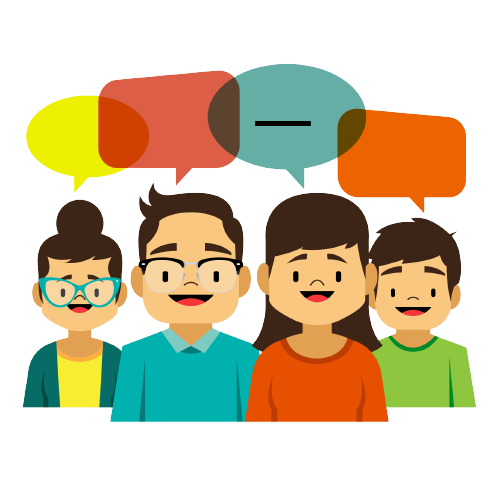
\includegraphics[width=\textwidth]{./media/image18a.png}
\end{center}

Verbos de elocução auxiliam a introdução de uma fala, 
indicando as atitudes e ações das personagens. 

Veja um exemplo a seguir.

\begin{myquote}
João disse:\\
--- Brisa é uma gatinha muito fofa!
\end{myquote}

Além disso, é no discurso direto que o narrador mais tem chance de mostrar
possíveis variedades da língua.

Já o \textbf{discurso indireto} consiste em uma reprodução do conteúdo das falas das
personagens, em vez de uma transcrição exata delas, com as palavras do
narrador. Ele atua como intermediário, muitas vezes incluindo também
emoções, reações, sentimentos ou marcas de personalidade do personagem.
Os verbos de elocução também aparecem, mas a estrutura é diferente.
Veja um exemplo a seguir.

\begin{myquote}
João disse que Brisa é uma gatinha muito fofa.
\end{myquote}
}

\section*{Atividades}

Leia o conto a seguir, de Monteiro Lobato, e resolva as atividades de 1 a 8.

%https://pixabay.com/pt/vectors/tartaruga-animal-desenho-animado-151431/


\begin{myquote}
\textbf{O cágado na festa do céu}

Certa vez houve uma grande festa no céu, para a qual foram convidados os
bichos da floresta. Todos se encaminharam para lá, e o cágado também, mas
ele era vagaroso demais, de modo que andava, andava e não chegava
nunca.

%\begin{wrapfigure}{r}{.4\textwidth}
\begin{center}
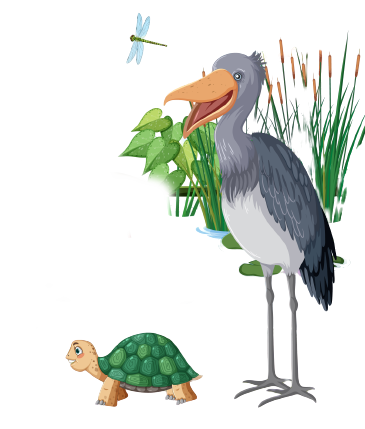
\includegraphics[width=.3\textwidth]{./media/image19a.png}
\end{center}
%\end{wrapfigure}

A festa era só de três dias, e o cágado nada de chegar. Desanimado, pediu
a uma garça que o conduzisse carregado nas costas. A garça respondeu: ``Pois não'', e
o cágado montou.

A garça foi subindo, subindo, subindo; de vez em quando perguntava ao
cágado se estava vendo a terra.

--- Estou, sim, mas lá longe.

A garça subia mais e mais.

--- E agora?

--- Agora já não vejo o menor sinalzinho da terra.

A garça, então, que era uma malvada, fez uma reviravolta no ar,
derrubando o cágado. Coitado! Começou a cair com velocidade cada vez
maior. Enquanto caía, murmurava:

\begin{verse}
\emph{Se eu desta escapar,}\\
\emph{léu, léu, léu,}\\
\emph{se eu desta escapar,}\\
\emph{nunca mais ao céu me deixarei levar.}\\
\end{verse}

Nisto, avistou lá embaixo a terra. Gritou:

--- Distanciem-se, pedras e paus, senão eu os esmagarei! As pedras e os paus
se afastaram e o cágado caiu. Mesmo assim arrebentou-se todo, em cem
pedaços.

Quem via tinha dó do coitado. Afinal de contas, aquela
desgraça tinha acontecido só porque o cágado teimou em comparecer à festa do
céu. De pena, um ser mágico da floresta juntou os pedacinhos.
É por isso que o cágado tem a casca feita de pedacinhos emendados uns
nos outros.

\fonte{Monteiro Lobato. O cágado na festa do céu. Adaptado.}
\end{myquote}

%\coment{Se os alunos não souberem, explique que o cágado é um animal parecido com uma tartaruga ou com um jabuti.}

\num{1} Quais são as personagens da história?

\reduline{Garça, cágado e um ser mágico da floresta.\hfill}
\linhas{1}

\num{2} Qual é o local onde se passa a história?

\reduline{Na terra e no céu.\hfill}
\linhas{1}

\num{3} Por que o cágado não chegava nunca à festa?

\reduline{Por que era vagaroso demais.\hfill}
\linhas{1}

\num{4} Por que o cágado teve a casca feita de pedacinhos emendados uns nos
outros?

\reduline{Isso aconteceu, porque um ser mágico teve dó 
do que aconteceu com o cágado e juntou outra vez os pedaços.\hfill}


% \num{5} Quem conta a história? Assinale a alternativa correta.

% \begin{boxlist}
% \boxitem{\white{X}} Um narrador que participa da história -- narração em primeira pessoa.

% \boxitem{X} Um narrador que não participa da história -- narração em terceira pessoa.
% \end{boxlist}


\num{5} No trecho a seguir, quem está participando do diálogo?

\begin{myquote}
A garça foi subindo, subindo, subindo; de vez em quando perguntava ao
cágado se estava vendo a terra.

--- Estou, sim, mas lá longe.

A garça subia mais e mais.

--- E agora?

--- Agora já não vejo o menor sinalzinho da terra.
\end{myquote}

\reduline{A garça e o cágado.\hfill}
\linhas{1}

\num{6} Em sua opinião, como seria a história se o diálogo apresentado no trecho selecionado na atividade anterior fosse formado
somente pelas falas dos personagens, sem a intervenção do narrador?

\reduline{Resposta pessoal. Espera-se que os alunos respondam que o leitor não
saberia de que forma os personagens falaram, uma vez que não existiriam
os comentários.\hfill}
\linhas{3}

\num{7} Ainda sobre o trecho selecionado na atividade 6, qual é o efeito expresso pelo discurso direto?

\reduline{O discurso direto apresenta ao leitor a conversa dos personagens como se estivesse ocorrendo naquele momento.\hfill}
\linhas{4}

Leia o diálogo, a seguir, e responda aos itens 8, 9 e 10.

\begin{myquote}
\begin{center}
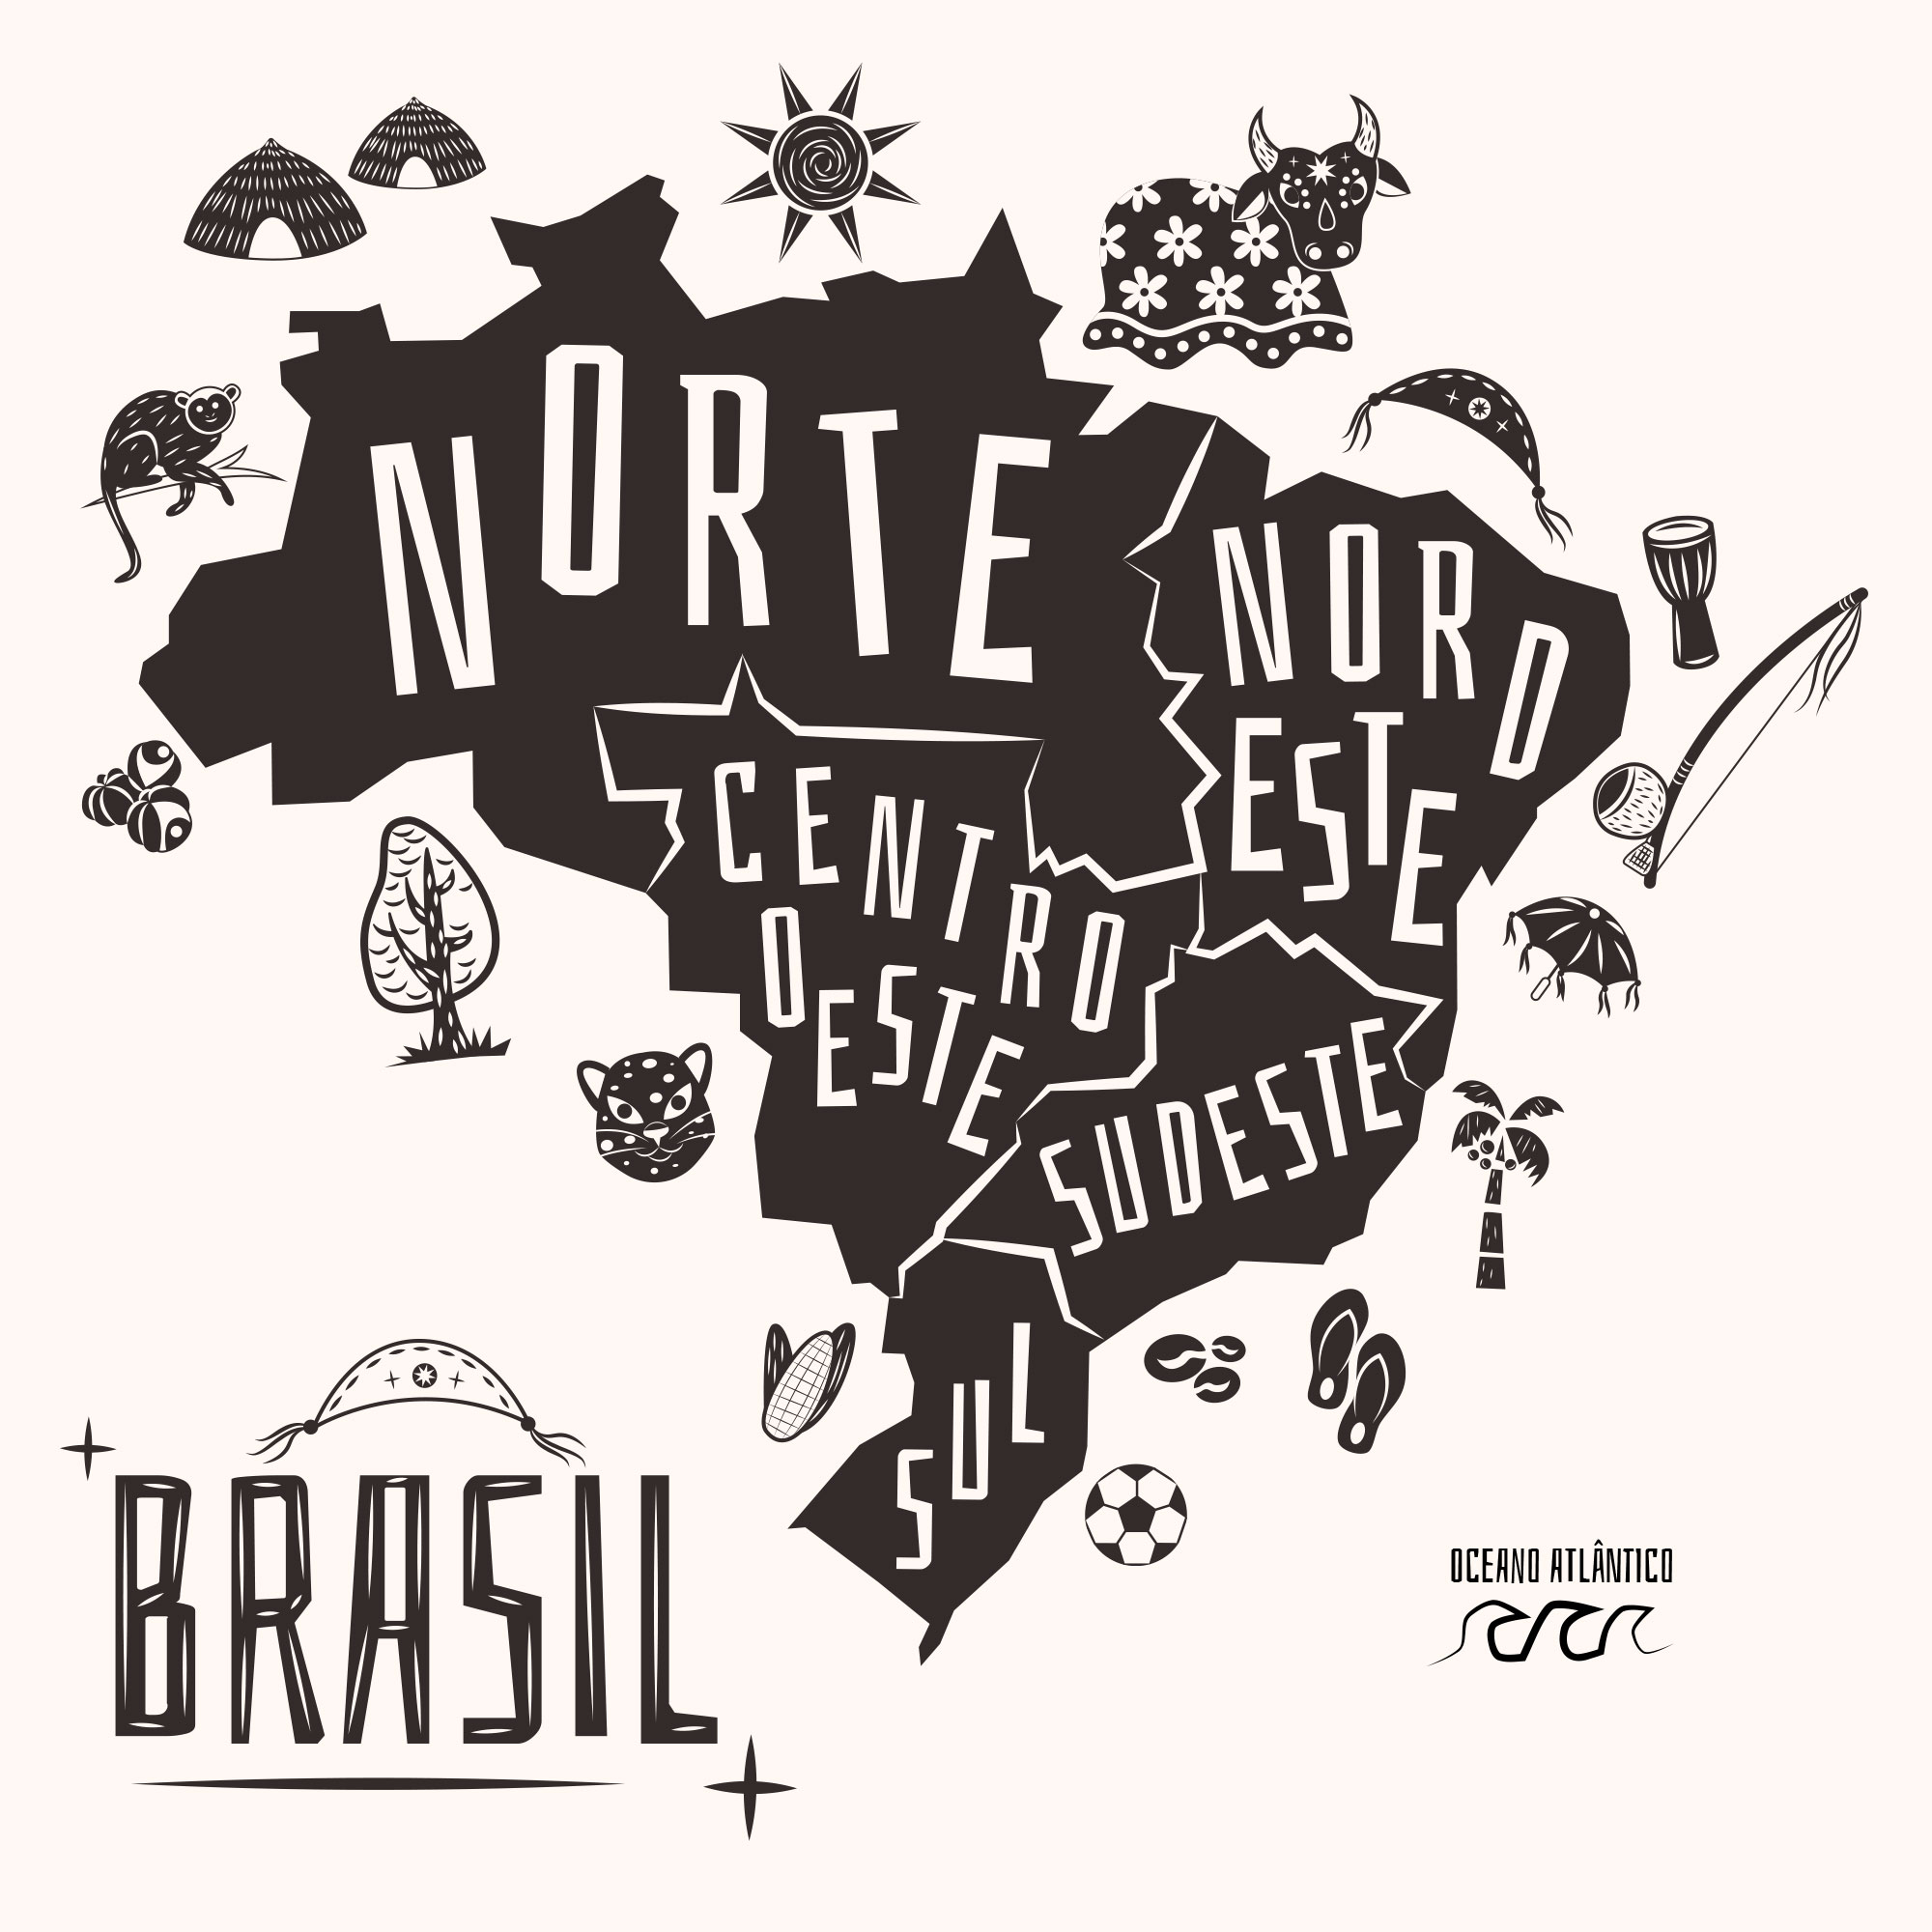
\includegraphics[width=.8\textwidth]{./media/image19c.jpeg}
\end{center}

Jandira encontrou Arnaldo na rua depois da aula de variantes linguísticas regionais 
e disse:

--- Arnaldo, sabia que lá em casa meu pai chama meu irmão de piá.

--- Ah, é? --- espantou-se Arnaldo. E por quê?

--- É que meu pai é do Rio Grande do Sul do Brasil 
e lá na onde ele nasceu é costume chamar menino de piá.

--- Meu pai, às vezes, me chama de menino, 
diz Arnaldo murmurando para si.

Nesse momento, chegam os pais de Jandira e Arnaldo, os dois riem e vão para casa.   

\fonte{Texto elaborado para este material}
\end{myquote}

\num{8} Qual o assunto da conversa entre Jandira e Arnaldo? 

\reduline{Jandira e Arnaldo conversam a respeito do assunto da aula: variantes linguísticas. De maneira mais específica, os alunos podem dizer que as personagens conversam sobre as diferentes palavras que são usadas para designar menino nas diferentes regiões do Brasil.}

\num{9} Variedade linguística regional refere-se às diferenças 
de vocabulário, pronúncia, entonação de uma língua em todos 
os lugares em que ela é falada. 

\begin{escolha}
\item Qual o Estado de origem do pai de Jandira?
\reduline{Rio Grande do Sul.\hfill}
\linhas{2}

\item Como o pai de Jandira chama o irmão dela?
\reduline{Piá.\hfill}
\linhas{2}

\item Como o pai de Arnaldo o chama?
\reduline{Menino.\hfill}
\linhas{2}
\end{escolha}

\num{10} Mandioca, mandioca-doce, mandioca-mansa, macaxeira, aipim. 
\begin{center}
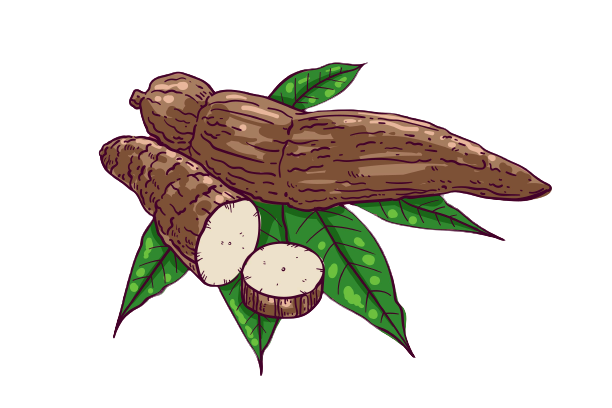
\includegraphics[width=\textwidth]{./media/image19b.png}
\end{center}

Qual o nome mais usado para mandioca na região onde você vive?
\reduline{Resposta pessoal. Procure mostrar aos alunos as diferenças, 
valorizando a variante usada e destacando que as diferenças 
estão relacionadas ao modo como a língua portuguesa 
se desenvolveu em cada região.\hfill} 
\linhas{3}

% \pagebreak
% Leia a piadinha a seguir para resolver as atividades de 9 a 11.

% %Inserir imagem ao lado do texto: https://cdn.pixabay.com/photo/2017/07/18/21/09/ice-cream-2517064\_960\_720.png


% \begin{myquote}
% \textbf{Sorvete de macaxeira}

% \begin{wrapfigure}{r}{.3\textwidth}
% 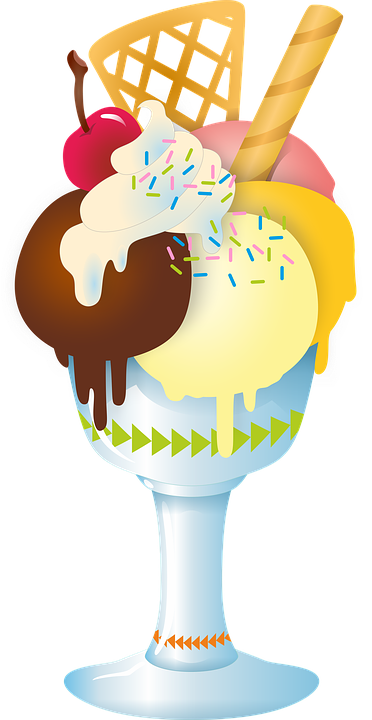
\includegraphics[width=.3\textwidth]{./media/image20.png}
% \end{wrapfigure}

% O garoto chega na sorveteria e pergunta:

% --- Tem sorvete de macaxeira?

% O vendedor responde:

% --- Não.

% No dia seguinte:

% --- Tem sorvete de macaxeira?

% --- Não.

% No outro dia:

% --- Tem sorvete de macaxeira?

% --- Não.

% No outro dia:

% --- Tem sorvete de macaxeira?

% --- Tem!

% --- Eca!

% \fonte{Domínio público.}
% \end{myquote}

% \num{8} Qual é a finalidade desse texto?

% \reduline{O gênero textual anedota é humorístico e tem por objetivo provocar o riso no
% leitor.\hfill}


% \num{9} Releia o trecho a seguir.

% \begin{myquote}
% O garoto chega na sorveteria e pergunta:

% --- Tem sorvete de macaxeira?

% O vendedor responde:

% --- Não.
% \end{myquote}

% \begin{escolha}[itemsep=-5pt]
% \item Quais são os verbos que introduzem as falas dos personagens? 
% \item\reduline{Os verbos são ``perguntar'' (na forma ``pegunta'') e ``responder'' (na forma ``responde''.\hfill}
% \linhas{1}


% \item Forme dupla com um colega e reescreva o trecho usando o discurso
% indireto.
% \item\reduline{Sugestão de resposta: O garoto chega na sorveteria e pergunta
% ao vendedor se tem sorvete de macaxeira. O vendedor responde que não.\hfill}
% \linhas{3}
% \end{escolha}

% \num{10} O nome de um vegetal muito usado no Brasil tem variações ao longo do território.
% Na piada, aparece o nome \textbf{macaxeira}. Você reconhece essa forma? Se sim, que outros
% nomes esses vegetal recebe? Se não, pesquise e escreva como esse vegeral é conhecido por
% você?

% \reduline{Os nomes são mandioca, macaxeira e aipim.\hfill}
% \linhas{1}

\section*{Treino}

Leia o texto para responder às questões 1 e 2.

\begin{myquote}
\textbf{Cinderela}

Há muito tempo, aconteceu que a esposa de um rico
comerciante adoeceu gravemente e, sentindo seu fim se
aproximar, chamou sua única rebenta e disse:

--- Minha querida, continue piedosa e boa menina que
Deus a protegerá sempre. Lá do céu olharei por você e estarei
sempre a seu lado.

Mal acabou de dizer isso, fechou os olhos e morreu.

A jovem ia todos os dias visitar o túmulo da mãe,
sempre chorando muito.

Veio o inverno, e a neve cobriu o túmulo com seu alvo
manto. Chegou a primavera, e o sol derreteu a neve. Foi então
que o viúvo resolveu se casar outra vez.

A nova esposa trouxe suas duas filhas, ambas louras e
bonitas --- mas só exteriormente. As duas tinham a alma feia
e cruel.

A partir desse momento, dias difíceis começaram para
a pobre enteada.

{[}...{]}

\fonte{Cinderela. Disponível em: \emph{www.dominiopublico.gov.br/download/texto/me000589.pdf}.
Acesso em: 18 abr. 2023. (Adaptado.)}
\end{myquote}

\num{1} A palavra ``rebenta'', que aparece no texto, é uma variação de

\begin{escolha}[itemsep=-5pt]
\item ``arrebenta''.

\item ``rebento''.

\item ``filha''.

\item ``broto''.
\end{escolha}

\num{2} Na linguagem coloquial, é mais usada a forma ``loiras'', palavra que tem uma variante no texto. Essa variante é

\begin{escolha}[itemsep=-5pt]
\item mais antiga.

\item mais correta.

\item menos usada na escrita.

\item mais comum no dia a dia.
\end{escolha}

\num{3} Leia o texto a seguir e responda ao item.

\begin{myquote}
Um compadre chega na casa do outro, que assistia à TV. Bate nas costas do amigo e pergunta:

--- E aí, cumpadi, firme?

O outro compadre responde:

--- Não, cumpadi. É futebor.

\fonte{Domínio público.}
\end{myquote}

O humor da piada se deve ao fato de que

\begin{escolha}[itemsep=-5pt]
\item os dois compadres utilizam variantes diferentes da língua.

\item o segundo compadre não reconheceu a palavra ``firme'', dita pelo outro.

\item o primeiro compadre não sabia que programa era aquele a que o amigo assitia na TV quando ele chegou.

\item houve uma confusão entre ``firme'' e ``filme'', porque as duas palavras são pronunciadas da mesma maneira.
\end{escolha}

\chapter{Adjetivos e advérbios}
\markboth{Módulo 7}{}

%Neste módulo, os alunos vão identificar adjetivos em textos e os substantivos a que se referem, assim como relacionar substantivos e adjetivos, observando a concordância de gênero e número.

\section{Habilidades do SAEB}

\begin{itemize}
  \item Analisar os efeitos de sentido decorrentes do uso dos adjetivos.
  \item Analisar os efeitos de sentido decorrentes do uso dos advérbios.
\end{itemize}

\subsection{Habilidades da BNCC}

\begin{itemize}
  \item EF03LP09, EF03LP23.
\end{itemize}

\conteudo{
Você provavelmente já notou que tudo o que existe no planeta
tem um nome. Imagine a seguinte situação: você está sentado no sofá da sala,
olhando para a televisão, e a televisão provavelmente está na
estante. Tudo isso tem um nome específico.

A palavra que nomeia algo é o \textbf{substantivo}, mas, muitas vezes,
para caracterizar melhor o que dizemos ou escrevemos, é preciso
qualificar os substantivos. A palavra que qualifica um substantivo é o
\textbf{adjetivo}.

A palavra ``cachorro'' é um substantivo que dá nome a um animal
doméstico, e muitas características podem ser atribuídas ao ``cachorro'':
``branco'', ``fofo'', ``bravo'', ``engraçado'', por exemplo.

Outro tipo de palavra que se liga sempre a uma outra é o \textbf{advérbio},
que pode modificar um \textbf{verbo}, um \textbf{adjetivo} ou um \textbf{outro
advérbio}. Em uma frase como ``O cachorro correu demais e cansou'', o advérbio
``demais'' modifica a forma verbal ``correu''. Já em uma frase como ``O cachorro
está muito feliz'', o advérbio ``muito'' modifica o adjetivo ``feliz''. Por fim,
em uma frase como ``O cachorro ficou bem mais contente'', o advérbio ``mais''
modifica o adjetivo ``contente'' e é modificado pelo advérbio ``bem''.
}

\section{Atividades}

Leia a carta de um leitor publicada em uma revista especializada em
divulgação científica dirigida a crianças. Depois, resolva as atividades de 1 a 7.

\begin{myquote}
\textbf{Lagartos}

\begin{wrapfigure}{r}{.3\textwidth}
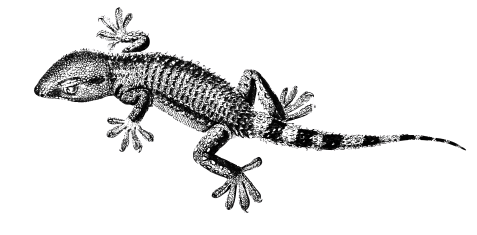
\includegraphics[width=.5\textwidth, angle=-95]{./media/image19d.png}
\end{wrapfigure}

Olá, equipe da CHC [Ciência Hoje das Crianças]! 

Ficamos extremamente impressionados com o artigo 
``Por que o lagarto balança tanto a cabeça?'' 
publicado na edição 244 da CHC. O artigo aborda 
o comportamento do lagarto-cinzento, que utiliza 
sua cabeça para se comunicar com outros membros 
da mesma espécie, informando seu gênero. 
Esses répteis habitam uma variedade de ambientes naturais, 
incluindo rochas, águas subterrâneas, solo e árvores. 
Apreciamos muito o texto e ficaríamos muito felizes 
se nossa carta fosse selecionada para publicação. 

Abraços cordiais.

Alunos do 3º ano da Escola Municipal Professor João Oliveira Lima. Pontal, Quixeré-Ce.

\fonte{Fonte de pesquisa: CHC. Lagartos. Fala Aqui! Disponível em:
\url{https://chc.org.br/artigo/fala-aqui/#:textasciitilde:text=Ficamos\%20muito\%20impressionados\%20com\%20o,se\%20s\%C3\%A3o\%20machos\%20ou\%20f\%C3\%AAmeas}.
Acesso em: 21 fev. 2023.}
\end{myquote}

\num{1} Qual é o assunto da carta?

\reduline{Os alunos ficaram muito impressionados
com o texto ``Por que o lagarto balança tanto a cabeça?'', publicado na
CHC 244, que fala sobre o lagarto-cinzento.\hfill}
\linhas{1}

\num{2} A quem a carta foi destinada?

\reduline{A carta foi destinada à equipe da revista CHC.\hfill}
\linhas{1}

\num{3} Quem é o remetente da carta?

\reduline{São os alunos do 3º ano da Escola Municipal Professor João Oliveira Lima. 
Pontal, Quixeré-Ce.\hfill}
\linhas{1}

\num{4} Transcreva o trecho da carta em que os leitores expressam sua opinião.

\reduline{Ficamos extremamente impressionados com o artigo 
``Por que o lagarto balança tanto a cabeça?'' publicado na
 edição 244 da CHC.\hfill}
 \linhas{1}

\num{5} Do trecho que você transcreveu, 
que adjetivo e que advérbio são responsáveis 
por demonstrar a opinião positiva dos leitores da revista?

\reduline{O adjetivo é ``impressionados'', modificado pelo advérbio ``extremamente''.\hfill}
\linhas{1}

\num{6} Como esse adjetivo e esse advérbio se relacionam entre si?

\reduline{O advérbio modifica o adjetivo.\hfill}
\linhas{1}

\num{7} Sobre o adjetivo que você identificou na atividade anterior, que outro adjetivo poderia substituí-lo sem alteração de sentido?
\linhas{1}

\reduline{Resposta pessoal. Sugestão de resposta: maravilhados.\hfill}
\linhas{1}

Leia o trecho do poema ``Meiguice'', de Adelina Lopes Vieira, para resolver as atividades de 8 a 10.

\begin{myquote}
\begin{minipage}{.5\textwidth}
%Inserir imagem ao lado do texto: \url{https://pixabay.com/pt/illustrations/gato-filhote-de-cachorro-7347316/}
\textbf{Meiguice}

{[}...{]}

Deram à linda Clarisse\\
uma gatinha mimosa,\\
tão branca, tão carinhosa,\\
tão engraçada, tão mansa\\
que a encantadora criança\\
por nome lhe pôs Meiguice.

{[}...{]}
\end{minipage}
\begin{minipage}{.5\textwidth}

\includegraphics[width=\textwidth]{./media/image23.png}
\end{minipage}

\fonte{Adelina Lopes Vieira. Meiguice. Disponível em:
\emph{http://www.dominiopublico.gov.br/download/texto/wk000075.pdf}.
Acesso em: 21 fev. 2023.}
\end{myquote}

\num{8} Que nome Clarisse deu à gatinha que ganhou?

\reduline{Meiguice.\hfill}

\num{9} Por que Clarisse deu esse nome à gatinha?

\reduline{Clarisse deu esse nome, porque a gatinha era branca, carinhosa, engraçada e mansa.\hfill}

\num{10} Que adjetivos aparecem no texto? E que advérbio?

\reduline{Os adjetivos são: ``linda'', ``mimosa'', ``branca'', ``carinhosa'', ``engraçada'', ``mansa'' e ``encantadora''. O advérbio é ``tão''.\hfill}
\linhas{1}

% \num{3} Relacione os substantivos aos adjetivos que podem caracterizá-los.
% \begin{multicols}{2}
% \red{ruas} 
% \red{sapato} 
% \red{bolo} 

% \red{cachorro} 

% \red{vestido} 

% \red{cabelo}

% \blue{quentinho}

% \blue{peludo}

% \blue{esburacadas}

% \blue{alto}

% \blue{ruivo}

% \blue{curto} 
% \end{multicols}

\section*{Treino}

\num{1} Leia um trecho de um conto popular.

\begin{myquote}
\textbf{A guardadora de patos}

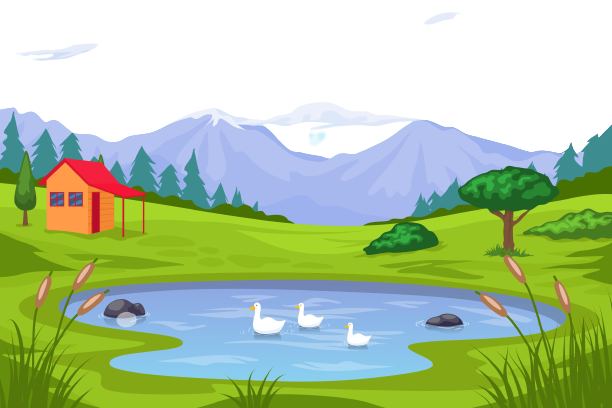
\includegraphics[width=\textwidth]{./media/image23a.png}

Era uma vez uma velha, muito velhinha, toda corcovada, que vivia com o
seu bando de patos num lugar deserto, no meio das montanhas, onde tinha
uma linda casinha. O sítio estava cercado de uma grande floresta [aonde] a
velha ia todas as manhãs, servindo-se de uma muleta para poder andar.
Trabalhava ali horas e horas com uma força extraordinária para a sua
idade; cortava a erva para os patos, que muito gostavam disso
{[}...{]}.

\fonte{Irmãos Grimm. Contos dos Irmãos Grimm. Rio de Janeiro: Livraria Garnier,
1932, p. 7. Disponível em: \emph{https://digital.bbm.usp.br/handle/bbm/7812}.
Acesso em: 22 fev. 2023.}

\begin{small}
\textbf{Vocabulário:} corcovada: corcunda.
\end{small}
\end{myquote}

Uma das palavras que, no texto, caracterizam a guardadora de patos é

\begin{escolha}[itemsep=-5pt]
\item ``deserto''.

\item ``velhinha''.

\item ``linda''.

\item ``grande''.
\end{escolha}



\num{2} Leia uma carta do leitor.

\begin{myquote}
\textbf{Fama de guloso}

\begin{wrapfigure}{r}{.4\textwidth}
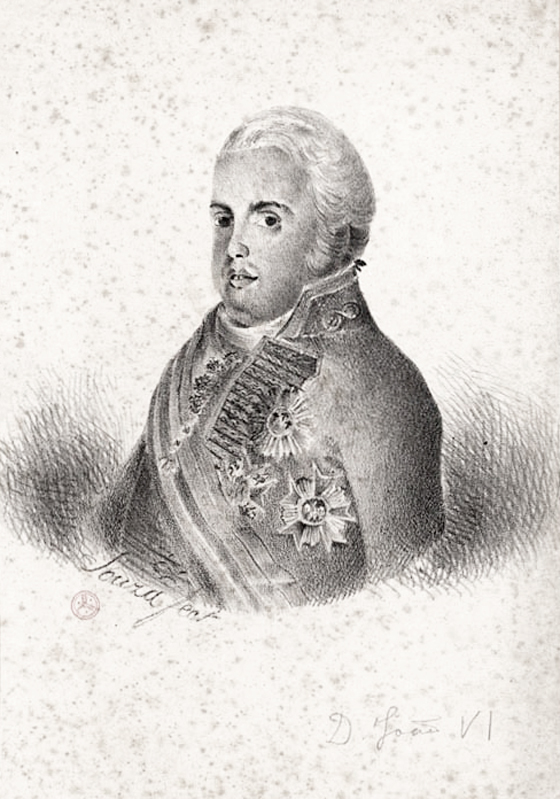
\includegraphics[width=.4\textwidth]{./media/image23b.jpg}
\end{wrapfigure}

Nós, estudantes do quinto ano, tivemos a oportunidade de ler um texto sobre a fama de D. João VI como um homem guloso. Achamos essa curiosidade muito interessante e entendemos por que os artistas o retrataram como um indivíduo mais gordinho nos retratos e nos livros de história. Ficamos imaginando as festividades que o rei costumava promover naquela época.

% Fama de guloso
% Somos alunos do 5º ano. Lemos um texto sobre a fama de D. João VI de ser guloso. Gostamos muito dessa curiosidade e compreendemos por que os artistas o retrataram gordinho nos quadros e nos livros de história. Imaginamos as festas que o rei promovia naquela época e toda a comilança dos convidados. Muitos assados, doces e bebidas. Guloso ou não, D. João VI contribuiu com nossa história.
% Alunos do 5º ano C. Escola Estadual José Ariano Rodrigues. Lins/SP.
% %Por que os textos das cartas foram alterados?

\fonte{Fonte de pesquisa: CHC. Fama de guloso. Fala aqui! Disponível em:
\emph{http://chc.org.br/artigo/fala-aqui-303/}. Acesso em: 22 fev. 2023.}
\end{myquote}

Uma das características de D. João VI citadas no trecho é que ele era

\begin{escolha}[itemsep=-5pt]
\item bonito, segundo os retratos da época.

\item guloso, segundo os estudantes do quinto ano.

\item famoso, já que ele era o rei de Portugal.

\item festeiro, promovendo muitas festas naquele época.
\end{escolha}



\num{3} Leia uma carta de leitor e a resposta que ela recebeu por parte da revista.

\begin{myquote}
\textbf{Cabeça de jacaré}

\begin{center}
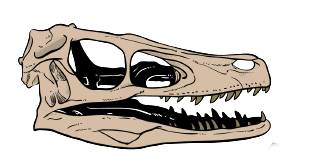
\includegraphics[width=.5\textwidth]{./media/image23c.png}
\end{center}

Na última edição da revista, tinha um texto sobre a cabeça do jacaré.
Muito legal! Mas fiquei pensando: como a gente sabe que o crânio do jacaré
é mais longo que o crânio do crocodilo?

\textit{Oi, Pedro! Quem dá as informações para os textos da CHC são cientistas.
Cada um é especializado em uma área. O texto que você leu veio de um
especialista em crocodilos e jacarés. Até a próxima!}

\fonte{Fonte de pesquisa: CHC. Cabeça de jacaré. Fala aqui! Disponível em:
\emph{http://chc.org.br/artigo/fala-aqui/}. Acesso em: 22 fev. 2023.}
\end{myquote}

No texto, o advérbio ``mais'' é responsável por

\begin{escolha}[itemsep=-5pt]
\item alterar o sentido de outro advérbio.

\item qualificar um substantivo.

\item criar uma comparação de superioridade.

\item diminuir a força do sentido de um adjetivo.
\end{escolha}